\documentclass[a4paper,notoc,openany]{tufte-book}%{scrreport}
%\usepackage[fontsize=11pt]{fontsize}
\usepackage{graphicx}
%\usepackage{draftwatermark}
\usepackage{amsfonts}
\usepackage{amsthm}
\usepackage{amsmath}
\usepackage{amssymb}
\usepackage{thmtools}
\usepackage{libertine}
\usepackage[libertine]{newtxmath}
\usepackage[T1]{fontenc}
\useosf
%\linespread{1.05}
%\usepackage{marginnote}
%\renewcommand{\marginfont}{\tiny\textit}
\usepackage[linesnumbered,ruled]{algorithm2e}
\usepackage{xfrac}
%\usepackage[dvipsnames,table]{xcolor}
\usepackage{tikz}
\usetikzlibrary{shapes.misc, automata, positioning, arrows}
\usepackage{xr-hyper} %for using references to lemmas/theorems from other documents.
\usepackage{hyperref}
\hypersetup{
	colorlinks=true,
	linkcolor=MidnightBlue,
	citecolor=Aquamarine}
%\usepackage{etoc}

\geometry{
  textwidth=28pc, left=0.75in
}


\titleformat{\section}%
{\normalfont\Large\itshape\color{PineGreen}}
{\thesection}
{1em}
{}
[]

\titleformat{\chapter}
{\huge\rmfamily\itshape\color{Sepia}}
{\thechapter}
{1em}
{}
[]

\titleformat{\subsection}
{\normalfont\rmfamily\itshape\color{PineGreen}}
{\thesubsection}
{1em}
{}
[]


\usepackage{scribe}
\usepackage{array}
\usepackage{enumerate}
\usepackage{blkarray, bigstrut}

\setcounter{secnumdepth}{2} % Add section/chapter numbers

%\SetWatermarkText{DRAFT}
%\SetWatermarkScale{0.7}
%\SetWatermarkColor[gray]{.95}

\tikzset{->,  % makes the edges directed
  >=stealth, % makes the arrow heads bold
	node distance=3cm, % specifies the minimum distance between two nodes. Change if necessary.
	every state/.style={thick, fill=gray!10}, % sets the properties for each ’state’ node
	initial text=$ $, % sets the text that appears on the start arrow
}


%uncomment the line below if you want references from week1.tex
%\externaldocument{week1} 

%%%% You can give your definitions here
\newcommand{\R}{\mathbb{R}}
\newcommand{\E}{\mathbb{E}}
\newcommand{\F}{\mathbb{F}}
\newcommand{\N}{\mathbb{N}}
\newcommand{\Z}{\mathbb{Z}}
\newcommand{\GF}{\mathbb{GF}}
\newcommand{\vect}[1]{\mathbf{#1}}
\DeclareMathOperator{\Var}{Var}
\DeclareMathOperator{\zeroes}{zeroes}
\DeclareMathOperator{\poly}{poly}
\DeclareMathOperator{\Det}{Det}
\DeclareMathOperator{\Cov}{Cov}
\DeclareMathOperator{\opt}{OPT}
\newcommand{\blank}{\sqcup}
\newcommand{\lang}[1]{\mathsf{#1}}
\newcommand{\marker}{\textsf{Marker} }
\newcommand{\dist}[1]{\mathbf{#1}}
\newcommand{\ranking}{{\textsf{RANKING}} }
\newcommand{\comp}[1]{\overline{#1}}
\newcommand{\set}[1]{\{1,2,\ldots,#1\}}
\newcommand{\coll}{\textsf{Coll}}
\DeclareMathOperator{\rem}{mod}
%%%%%%%%%%%%%%%%%%%%

\newlength{\drop}
\setcounter{tocdepth}{1}

\newcommand*{\titleS}{\begingroup% Scripts, T&H p 151
  \drop = 0.1\textheight \vspace*{\drop}
  {\Huge \textsc{Randomized Algorithms}}\\[\baselineskip]
  {\Large CS 6170}\\[\baselineskip]
  \vfill
  \rule{0.4\textwidth}{0.4pt}\\[\baselineskip]
  {\Large\itshape Dept. of Computer Science and Engineering\\ IIT Madras}\par
	\vspace*{\drop}
	\endgroup}

%\title{\Huge Randomized Algorithms\\ \noindent \Large CS 6170}
%\date{CS 6170}
%%\author{Yadu Vasudev}
%\publisher{\Large Department of Computer Science and Engineering\\ \noindent IIT Madras}
%

\begin{document}

\titleS

%\maketitle

%\newpage
\tableofcontents
\chapter*{Preface}

These are the notes for the Randomized Algorithms course that was offered in
July - Nov 2021 and 2022. The material that is covered here is not new, and
there are a number of references available for these topics. I prefer the presentation of a particular topic better in one book
than in another. Therefore, even though the material covered is basic, I have
not restricted myself to one textbook. These notes collate the many different
expositions and tries to make a consistent presentation. Many thanks to the
students who took this course in 2021 and 2022 and scibed many of the
lectures. I have generously borrowed from the scribed notes.

These notes are not proof-read and may contain errors. If you find any, please
email me.

\chapter{Introduction}

Randomization is ubiquitous in computer science. In many cases, we obtain faster, simpler and more elegant algorithms that better the "polynomial-time" algorithm known for the same problem. An example is the problem of primality testing. Suppose you are given an integer $n$ as input and you want to check if $n$ is prime or not. The trivial algorithm would be to check whether  some number between $1$ and $\sqrt{n}$ divides $n$ or not. This is highly inefficient since for a number with $100$ digits could be as large as $2^{100}$ and the naive algorithm has a running time for $2^{50}$. In a breakthrough result in 2002, AKS showed that there is a polynomial time algorithm for testing primality, and currently the best upper bound known is $O(\log^7 n)$. While this running time does not look as prohibitive as the naive algorithm, it is, nonetheless, not very practical. As it turns out, there is a very simple algorithm to test primality, albeit one that can make an error occassionally. We will make the statement "make an error occassionally" precise in a moment. But, let us first look at the algorithm known as the Miller-Rabin test.

\begin{algorithm}
	\KwIn{Integer $n$}
	\BlankLine
	
	Let $n = 2^rs+1$, where $s$ is odd
	
	Choose $a$ uniformly at random from $\{2, \ldots, n-1\}$
	
	\lIf{$a^{s} \neq 1$ (mod $m$)}{return \texttt{composite}}
	
	\For{$0 \leq i \leq s-1$}{
		\lIf{$a^{2^is}=-1$ (mod $m$)}{return \texttt{prime}}
	}

	return \texttt{composite}
	\caption{\textsc{Miller-Rabin Primality Test}}
	\label{alg:primality}
\end{algorithm}

By repeated squaring and computation of remainder modulo $n$, it is easy to see that the running time of the algorithm is $O(\log^2 n)$. As you can see, the algorithm is easy to implement in terms of the calculations that has to be done, and its running time is also good asymptotically. It can shown that if $n$ is a prime, then irrespective of the choice of $a$ then algorithm will always return "prime". When analyzing the algorithm (which is non-trivial and requires some basic algebra), we can show that for at least $3/4$th fraction of numbers between $2$ and $n-1$, the algorithm will return "composite". In other words, if the number is prime, then the probability that the algorithm errs is zero, whereas if it is composite, then the probability that it errs is at most $1/4$. It is possible to bring down with error probability to something as tiny as $1/2^40$ without changing the asymptotic complexity of the algorithm (we will see how to do this a little later). Note that while the algorithm is simple to explain, its proof of correctness will not be easy, in most cases. 

We will see various settings where randomized algorithms give simple, elegant and fast algorithms where fast deterministic algorithms are not known. Nonetheless, most theoretical computer scientists believe that randomness does not inherently add more computational power. In other words, they believe that if a computational problem has a fast randomized algorithm, then it also has a fast deterministic algorithm! Then why study randomized algorithms at all? Firstly, we are currently far away from that goal of converting every fast randomized algorithm to a fast deterministic algorithm. Secondly, fast here means polynomial-time. So, you could have a randomized primality test that runs in $O(\log^2 n)$ time and the best deterministic primality test may still require $O(\log^7 n)$. That is a considerable gap in many practical situations. Finally, there are scenarios where randomization is unavoidable. One such example is counting motifs in large graphs that are too big to run classical algorithms on. Any algorithm that can approximate these counts necessarily has to be randomized. 

In the rest of this lecture, we will see a few more examples while refreshing some basic concepts in discrete probability.

\section{Polynomial Identity Testing}

Suppose that you are given a degree-$d$ polynomial $p(x) = \sum_{i=0}^d c_i x^i$ in the explicit way. Your friend claims that the factorization of $p(x)$ is given by $q(x) = \prod_{i=1}^d (x-a_i)$ by using a program for polynomial factorization that she has written. How do you check if your friend is indeed telling the truth? The most straightforward way would be for you to expand the factorization $q(x)$ and check that it indeed gives $p(x)$. But, this is tedious since you might end up with far more terms than just the $d$ terms that you will then have to cancel and reduce. With the power of randomness there is something very simple that you can do!

Let us assume for the moment that the numbers involved are all rationals. Consider the polynomial $p(x) -q(x)$. Notice that this polynomial is identically zero precisely when $q(x)$ is the factorization of $p(x)$. Furthermore, $p(x) - q(x)$ is a degree-$d$ polynomials. Now, you know that every polynomial of degree $d$ has at most $d$ roots (this is known as the fundamental theorem of algebra). This gives you an idea for a solution! You choose a number $a$ uniformly at random from the set $\{1,2,\ldots,100d\}$, and check if $p(a)-q(a)=0$. Notice that if $q(x)$ is indeed the factorization of $p(x)$, then for every $a$, $p(a) - q(a)=0$ and we will answer correctly. Moreover, if $q(x)$ is not the correct factorization of $p(x)$, then $p(x)-q(x)$ is a non-zero polynomial of degree $d$. Hence, it has at most $d$ distinct roots, and the probability that $a$ is one such root is at most $1/100$.

A generalization of this problem is the famous \textit{Polynomial Identity Testing} problem (PIT for short). Here you have access to a multivariate polynomial $p(x_1, x_2, \ldots, x_n)$ of degree $d$. Observe that the number of monomials of this polynomial can be as large as $\binom{n+d-1}{n}$, and the polynomial is expressed succinctly as a product of a small number of polynomials. You want to check if this polynomial is identically zero. Since the explicit description of the polynomial can be exponentially larger than the given representation, it is inefficient to write out the full polynomial and check whether it is indeed zero. Once again randomness comes to our rescue! We will state a lemma that generalized the fundamental theorem of arithmetic.

\begin{lemma}
	[Lipton-DeMillo-Schwartz-Zippel]
	Let $p(x_1, x_2, \ldots, x_n)$ be a non-zero degree $d$ polynomial over rationals. Let $S$ be a subset of rational numbers. Then,
	\begin{align*}
		\Pr_{a_1, a_2, \ldots a_n \in_r S} \left[ p(a_1, a_2, \ldots, a_n) = 0  \right] &\leq \frac{d}{|S|}
	\end{align*} 
\end{lemma}

Here by ${a_1, a_2, \ldots, a_n \in_r S}$ we mean that each $a_i$ is picked from $S$ with replacement. We will use this notation through the lecture notes. Observe that when $n=1$, then the lemma follows from the fundamental theorem of algebra. The lemma can be proved by an induction on $n$ (the number of variables).

\chapter{Random variables and their properties}

The outcome of a randomized algorithm is a variable that depends on the random choices made by the algorithm during its execution. Analyzing the guarantees of a randomized algorithm amounts to analyzing the properties of this \emph{random variable}. Formally, a random variable is a function $X:\Omega \to \R$. The standard notational convention is to use capital letters to denote random variables. We can associate events with random variables in a very natural way. If a random variable $X$ takes a value $a$, then the event associated with this is the set $A \subseteq \Omega$ such that $\omega \in A$ iff $X(\omega) = a$. We will also write that 
\begin{align*}
	\Pr[X=a] = \sum_{\omega \in \Omega, X(\omega)=a} \Pr[\omega]. 
\end{align*}

While analyzing randomized algorithm, we will need to define suitable random variables based on the algorithm  at hand. In many cases, it will difficult to analyze the random variable corresponding to the output of the algorithm directly, and we may need to express it as a function of other random variables. One important type of random variables that we will see is the \emph{indicator random variable}. For an event $E\subseteq \Omega$, an indicator random variable $X_A$ takes values $1$ or $0$ depending on the occurrence of the event $A$. One of the most important parameters associated with a random variable is its \emph{expectation}. The expectation of a random variable is the average value taken by it. Formally, we have
\begin{definition}
	[Expectation]
	Let $\Omega$ be a sample space, and let $X:\Omega \to \R$ be a random variable. The expectation of the random variable $\E[X]$ is given by
	\begin{align*}
		\E[X] &= \sum_{\omega \in \Omega} \Pr[\omega] X(\omega).
	\end{align*}
	\label{defn:exp}
\end{definition}

Similar to the independence of events, we can define when two random variables are independent. We will say that two random variables $X$ and $Y$ are \emph{independent} if for every $x$ and $y$, we have
\begin{align*}
	\Pr[(X=x) \cap (Y=y)] = \Pr[X=x]\Pr[Y=y].
\end{align*}

An important property of expectation that will useful in analyzing random variables and algorithms is the following seemingly trivial property. The proof is a simple calculation from the definition, and is left as an exercise.
\begin{theorem}
	(Linearity of Expectation)
	Let $X_1, X_2, \ldots, X_n$ be any $n$ random variables, and let $X = \sum_{i=1}^n X_i$. Then, we have
	\begin{align*}
		\E[X] = \E\left[\sum_{i=1}^n X_i\right] = \sum_{i=1}^n \E[X_i].
	\end{align*}
	\label{thm:loe}
\end{theorem}
Notice that the statement makes no assumption about the properties of the random variables. With these ideas, we can already say something non-trivial about an important combinatorial problem.

\section{Maxcut}

In the mincut problem that we saw in the last lecture, our aim was to find the cut of smallest size in a graph $G$. Now, we ask the complement question: Given a graph $G$, find the cut of largest cardinality. It is a central problem in combinatorial optimization, and no efficient algorithms are known for it. The problem is NP-hard, and hence unlikely to have an efficient algorithm. Let us look at a simple randomized algorithm for this problem.

\begin{algorithm}
	\KwIn{Graph $G(V,E)$}
	
	Set $V_1, V_2 \gets \emptyset$
	
	\For{$u\in V$}{
		Choose $b$ u.a.r from $\{0,1\}$
		
		\leIf{$b=0$}{$V_1 \gets V_1 \cup \{u\}$}{$V_2 \gets V_2 \cup \{u\}$}
	}

	Output $X = |\{(u,v)\in E | u\in V_1, v\in V_2 \}|$.
	\caption{Max-Cut}
	\label{alg:maxcut}
\end{algorithm}

Firstly, if we analyze this algorithm with respect to a fixed cut $C$, then the probability that this cut size is output is $1/2^n$. If this probability was any better, then we could have repeated this for sufficient number of times and obtained a fast algorithm. What we will do instead is to look at the random variable $X$ and obtain some non-trivial bound on the size of the maxcuts of a graph. The output $X$ is a random variable that depends on the random choices made for the vertices in the graph. First, we show the following.

\begin{lemma}
	For $X$ output in Algorithm~\ref{alg:maxcut}, $\E[X] = |E|/2$.
	\label{lem:size-maxcut}
\end{lemma}
\begin{proof}
	For each edge $e\in E$, define the indicator random variable $X_e$ that denotes the event that $e$ is a cut-edge. We can then write 
	\begin{align*}
		X = \sum_{e\in E} X_e.
	\end{align*}
	By the linearity of expectation, $\E[X] = \sum_{e\in E} \E[X_e]$. So, all that remains now is to compute the expectation of $X_e$. For this we use the observation that for an indicator random variable, the expectation is equal to the probability of the occurrence of the corresponding event. In this case, we have $\E[X_e] = \Pr[\text{$e$ is a cut edge}]$. Suppose that $e=(u,v)$, then we have
	\begin{align*}
		\Pr[\text{$e$ is a cut edge}] &= \Pr[(u \in V_1 \text{ and } v\in V_2) \cup (u \in V_2 \text{ and } v\in V_1)]\\
		&= \Pr[(u \in V_1 \text{ and } v\in V_2)] + \Pr[(u \in V_2 \text{ and } v\in V_1)] \\ &= \frac{1}{2}.
	\end{align*}
	Consequently, $\E[X] = |E|/2$.
\end{proof}

Notice that the expectation here is a weighted mean over all the cut sizes. Consequently, if the weighted mean is greater than a number $r$, then there must actually exists such a cut of size at least $r$. In fact, this observation gives us the following highly non-trivial theorem about cuts in graphs.

\marginnote{
  This method of proving the existence of combinatorial objects using
randomization is known as the \emph{probabilistic method}. It is a very powerful
tool that can be used in a variety of settings that do not seem amenable to such
techniques on first sight.
}
\begin{theorem}
	Every graph $G$ with $m$ edges has a cut of size at least $m/2$.
	\label{thm:maxcut}
\end{theorem}


Let us try to understand the random variables $\{X_e\}_{e\in E}$ a little better. Firstly, for two edges $e_1$ and $e_2$, $X_{e_1}$ and $X_{e_2}$ are independent. If $e_1$ and $e_2$ don't share a vertex, then it is obvious. Suppose that $e_1$ and $e_2$ share a vertex $u$. Even in this case, if given that $X_{e_1}$ is $0$ or $1$, the value of $X_{e_2}$ depends on where the other endpoint is placed. Thus $\Pr[X_{e_2}=1 | X_{e_1}=1] = \Pr[X_{e_2}=1 | X_{e_1}=0] = 1/2$. Now suppose that the edges $e_1, e_2$, and $e_3$ for a triangle on vertices $u,v$, and $w$. Now give the values of $X_{e_1}$ and $X_{e_2}$, the positions of all three vertices are fixed, and hence the value of $X_{e_3}$. Thus, the variables $\{X_e\}_{e\in E}$ are not fully independent. The linearity of expectation gave us a non-trivial bound, even when we had no information about the properties of the random variables involved other than their expectation.

\subsection{Constructing a large cut deterministically}

We showed that a random partition of the vertices gives you a cut, that on expectation contains at least half of the edges in the graph. But, can you construct such a cut-set deterministically. Recall the analysis of the expectation. If you look at it carefully, you'll notice that we don't really require that the assignment of vertices to $V_1$ and $V_2$ need not be completely independent. For the analysis to go through, all we need is the following:
\begin{align*}
	\Pr[u \in V_1 \text{ and } v\in V_2] &= \Pr[u \in V_1] \Pr[v \in V_2], \\
	\Pr[u \in V_2 \text{ and } v\in V_1] &= \Pr[u \in V_2] \Pr[v \in V_1]
\end{align*}
Thus, what we actually need is just pairwise independence, rather than full independence for the analysis to go through. Instead of choosing the part for each vertex uniformly at random, we do the following.

Let $\vect{b} = b_1b_2\ldots b_k$ be a binary string such that $k=\log n$. We can associate subsets of $[k]$ with the $n$ vertices in the graph in a natural way. Let $S_u \subseteq [k]$ denote the set associated with vertex $u$. For a vertex $u$, we compute $b_u = \oplus_{i\in S_u} b_i$, and assign $u$ to $V_b$. Now, for any two $u$, $v$, the set $S_u$ and $S_v$ are different, and hence if $\vect{b}$ is chosen uniformly at random from $\{0,1\}^{\log n}$, the probability $\Pr[b_u \neq b_v] = 1/2$. Therefore, we can rewrite the maxcut algorithm as follows.

\begin{algorithm}
	\KwIn{Graph $G(V,E)$}
	
	Set $V_1, V_2 \gets \emptyset$
	
	Choose $b_1, b_2, \ldots, b_{\log n} \in_r \{0,1\}$
		
	\For{$u\in V$}{
		Compute $b = \oplus_{i\in S_u} b_i$
		
		Set $V_b \gets V_b \cup \{u\}$.
	}
	
	Output $X = |\{(u,v)\in E | u\in V_1, v\in V_2 \}|$.
	\caption{Max-Cut Modified}
	\label{alg:maxcut-modified}
\end{algorithm}

The analysis of this algorithm is identical to the original algorithm. But, now we can remove the randomness in the following way:

\begin{algorithm}
	\KwIn{Graph $G(V,E)$}
	
	Set $V_1, V_2 \gets \emptyset$
	
	\For{$\vect{b}=(b_1,b_2,\ldots,b_{\log n})$}{	
		
		\For{$u\in V$}{
			Compute $b = \oplus_{i\in S_u} b_i$
			
			$V_b \gets V_b \cup \{u\}$
		}
		Compute $X_{\vect{b}} = |\{(u,v)\in E | u\in V_1, v\in V_2 \}|$
	}
	
	Output $\max \{X_{\vect{b}}\}_{\vect{b} \in \{0,1\}^{\log n}}$

	\caption{Max-Cut Deterministic}
	\label{alg:maxcut-det}
\end{algorithm}

Since the expected value is at least $m/2$, the largest cut must have size at least $m/2$. Therefore, the output will be a cut of size at least $m/2$. Furthermore, the outer loop runs for $n$ steps, and hence we have a polynomial-time $1/2$-approximation algorithm.

\subsection{Method of conditional expectations}

The method of conditional expectations is a fairly generic way to derandomize a
lot of randomized algorithms. We will see it applied to our maxcut algorithm. As
the name suggests, we will write the expected value $\E[X]$ of the cut using
conditional expectations. Let us order the vertices $v_1, v_2, \ldots, v_n$. We
can consider the algorithm as taking vertices sequentially in this order and
putting them in one of the two parts $V_1, V_2$ uniformly at random. Thus, we can write the expectation $\E[X]$ as follows:
\begin{align*}
  \E[X] &= \E[X|v_1 \in V_1]\cdot \Pr[v_1 \in V_1] + \E[X|v_1 \in V_2]\cdot \Pr[v_1\in V_2]\\
  &= \frac{1}{2} \left( \E[X|v_1 \in V_1] + \E[X|v_1 \in V_2] \right)
\end{align*}

Since we know that $\E[X] \geq |E|/2$, either $\E[X|v_1\in V_1]$ or
$\E[X|v_1\in V_2]$ is at least $|E|/2$. If we find which of these is larger,
then we can put $v_1$ in the corresponding set and proceed further.
\marginnote{Actually you only want some good lower bounds for these conditional
  expectations that can be easily computed. These are called \emph{pessimistic
    estimators}.}
For making this method work, we need a way to compute these
conditional expectations.

Let us see how to compute $\E[X|v_1\in V_1]$. In this initial case, every edge
crosses the cut with probability exactly $1/2$. In other words, it doesn't
matter where you place $v_1$. Let us assume that we placed $v_1$ in the set
$V_1$. Consequently, $\E[X|v_1 \in V_1] \geq |E|/2$. In the next step, we can
use the conditional expectations once more to write the following:
\begin{align*}
  \E[X|v_1\in V_1] &= \E[X|v_1\in V_1, v_2\in V_1] \cdot \Pr[v_2\in V_1]~ +~ \\
                   &\qquad\qquad  \E[X|v_1\in V_1, v_2\in V_2] \cdot \Pr[v_2\in V_2]\\
 &= \frac{1}{2} \left(\E[X|v_1\in V_1, v_2\in V_1] + \E[X|v_1\in V_1, v_2\in V_2] \right)
\end{align*}

To compute $\E[X| v_1 \in V_1, v_2 \in V_1]$ we observe the following: if
$(v_1, v_2)\in E$, then $(v_1, v_2)$ is not in the cut and every other edge is
in the cut with probability $1/2$. Similarly, for
$\E[X|v_1\in V_1, v_2\in V_2]$, if $(v_1,v_2)\in E$ then it is in the cut and
every other edge is in the cut with probability $1/2$. In particular, we can see
that if $(v_1, v_2)\in E$ then the conditional expectation is maximized when
$v_2$ is placed in $V_2$.

In the $i^{th}$ step of this process, we want to find the $V_{b_i}$ such that
the conditional expection
$\E[X|v_1 \in V_{b_1}, v_2\in V_{b_2}, \ldots, v_i\in V_{b_i}]$ is
maximized. This can be computed since for every edge $(v_j,v_k)$ such that
$1\leq j,k\leq i$, it is already known whether it is in the cut or not. Every
other edge is in the cut with probability $1/2$. Just like before, to maximize
the conditional expectation, $v_i$ must be placed in the part $V_{b_i}$ that
maximizes the number of cut edges between itself and the vertices
$v_1, v_2, \ldots, v_{i-1}$.

This leads us to the following greedy algorithm: Order the vertices
$v_1, v_2, \ldots, v_n$ arbitrarily. For each $i$ in order, place $v_i$ in the
part that maximizes the cut edges incident on it and the previous $i-1$
vertices. The argument described above using conditionl expectations guarantees
that this process will give a cut of size at least $|E|/2$.

\section{Quicksort}
We use the ideas from the previous section to analyze a randomized version of the Quicksort algorithm. Recall that in the deterministic Quicksort algorithm, we choose a pivot element in the array (say, the last element) and then partition the array into two parts based on whether the numbers are smaller or larger than the pivot. Then we recursively sort the two parts to obtain the final sorted array. The running time depends on the choice of the pivot since we want the pivot to divide the array into two arrays of similar sizes. 

For instance, if the pivot is the largest element of the array each time, then the running time is $O(n^2)$. On the other hand, if we choose the median as the pivot at every step, then the running time is given by the recurrence
\begin{align*}
	T(n) = 2T\left( \frac{n}{2} \right) + O(n).
\end{align*}

Let us look at a randomized variant of Quicksort, where we choose a pivot element uniformly at random from the array. We hope that the algorithm will avoid the case of choosing a bad pivot at every step of the recursion. In this case, the running time of the algorithm, as measured by the number of comparisons that it makes, is a random variable. Let us analyze this random variable now.

For this, let $\vect{a} = a_1, a_2, \ldots, a_n$ be the array given and let $\vect{b} = b_1, b_2, \ldots, b_n$ be the sorted version of the array. We will argue with respect to this array $\vect{b}$. Let $X$ denote the total number of comparisons performed ny the Quicksort algorithm while converting the array $\vect{a}$ to $\vect{b}$. It will be hard to argue directly about $X$, so we will express $X$ as a function of random variables that are easier to analyze. 

To that end, let $X_{ij}$ denote an indicator random variable corresponding to the event that $b_i$ and $b_j$ are compared during the execution of randomized Quicksort. We can then write $X$ as
\begin{align*}
	X &= \sum_{1\leq i<j\leq n} X_{ij}, \text{ and hence, }\\
	\E[X] &= \sum_{1\leq i<j\leq n} \E[X_{ij}].
\end{align*} 
Since $X_{ij}$ is an indicator random variable, $\E[X_{ij}] = \Pr[\text{$b_i$ and $b_j$ are compared}]$. 

Let us try to analyse $X_{ij}$. Consider the elements $b_i \leq b_{i+1} \leq \ldots \leq b_j$. The only way that $b_i$ and $b_j$ are compared is that the first time a pivot is chosen from this interval, it is either $b_i$ or $b_j$. Since the pivot is chosen uniformly at random from the entire array, $E[X_{ij}] = \tfrac{2}{j-i+1}$. Thus we can write
\begin{align*}
	\E[X] &= \sum_{i=1}^{n-1} \sum_{j=i+1}^n \frac{2}{j-i+1}\\
	&= \sum_{i=1}^{n-1} \sum_{k=2}^{n-i+1}\frac{2}{k} = \sum_{k=2}^n \sum_{i=1}^{n+1-k} \frac{2}{k} = \sum_{k=2}^n (n+1-k)\frac{2}{k}\\
	&= 2(n+1)\sum_{k=2}^n \frac{1}{k} - 2(n-1)\\
	&= 2(n+1)\sum_{k=1}^n \frac{1}{k} - 4n
\end{align*}

The sum $\sum_{k=1}^n \frac{1}{k}$ is the harmonic sum and is equal to $\ln n +\Theta(1)$. Therefore, we have $\E[X] = 2n\ln n + \Theta(n)$. If you recall analysis of algorithms, this might seem a little unsatisfactory. It is true that on expecation, Quicksort is fast, but how is the random variable actually distributed? Is it the case that the running time can vary wildly, and yet the expectation is $\Theta(n\log n)$? Or is the actual running time concentrated closely around the expectation? That would be a more useful analysis. For now, we will leave it here, but do a more careful analysis once we develop a few more tools.

\section{Probability Mass Functions (PMF) and random variables}

Till now, we have been looking at randomized algorithms, and defined random variables based on the algorithm at hand. Another way to define random variables (without looking at any random experiment) is to define the corresponding probability mass function. We will see come distributions that arise in many different scenarios, and will be useful in the analysis of randomized algorithms. Let us start with the formal definition of a Probability Mass Function (PMF).

\begin{definition}
	Let $X$ be a random variable. The PMF associate with $X$ is a function $p_X:\R \to \R$ defined as follows:
	\begin{align*}
		p_X(u) = \Pr[X=u].
	\end{align*}
	\label{defn:pmf}
\end{definition}

Notice that the value $p_X(u)=0$ if $u$ is not in the range of $X:\Omega \to \R$. The events $\{X = u\}$ is a partition of $\Omega$, and hence $\sum_{u \in \text{range}(X)} p_X(u) = 1$. The PMF of a random variable gives you all the information you need to analyze the random variable $X$. While analyzing a randomized algorithm, we usually don't have access to the PMF directly, but there are some common PMFs that arise in different random process. 

\subsection{Binomial distribution}

A common random experiment that arises in many scenarios is the following. Consider an experiment that succeeds with probability $p$ and fails with probability $1-p$. We can associate an indicator random variable with this experiment that is $1$ iff the experiment succeeds. Such an indicator random variable is known as a Bernoulli random variable. A natural question that comes up in many situations is to count the number of successes in a run of $n$ iterations of this experiment. This random variable is known as the binomial random variable and the associated PMF is the binomial distribution.

\begin{definition}
	A random variable $X$ is a binomial random variable with parameters $n$ and $p$ if the PMF of the random variable $X$ is given by 
	\begin{align*}
		p_X(i) = \binom{n}{i} p^i (1-p)^{n-i}
	\end{align*}
	for $i \in \{0,1,\ldots,n\}$ and $0$ otherwise.
	\label{defn:binomial}
\end{definition}

Alternately, you can think of the binomial random variable being the sum of $n$ Bernoulli random variables, though the PMF defines the random variable completely as far as we are concerned. If we think of $X$ as the sum of $n$ Bernoulli random variables with parameter $p$, then by the linearity of expectation, we can easily conclude that $\E[X]=np$. If we were think of the binomial random variable purely in terms of its PMF, then we can explicitly compute its expectation as follows:
\begin{align*}
	\E[X] &= \sum_{i=0}^n i \binom{n}{i} p^i (1-p)^{n-i}\\
	&= \sum_{i=1}^n \frac{n!}{(i-1)!(n-i)!} p^i (1-p)^{n-i} = np\sum_{i=1}^n \frac{(n-1)!}{(i-1)!(n-i)!}p^{i-1}(1-p)^{n-i}\\
	&=np\sum_{j=0}^{n-1} \binom{n-1}{j}p^j(1-p)^{n-1-j} = np.
\end{align*}

\subsection{Geometric distribution}

Consider a Bernoulli trial with parameter $p$. We are interested in the number of trials that has to be performed before the first success. The random variable that counts this number is known as a geometric random variable.

\begin{definition}
	A random variable $X$ is said to be a geometric random variable with parameter $p$ if the PMF associated with $X$ is given by
	\begin{align*}
		p_X(i) = (1-p)^{i-1} p.
	\end{align*}
\end{definition}

Given the PMF, we can once again explicitly calculate the expectation from the definition.
\begin{align*}
	\E[X] &= \sum_{i\geq 1} i (1-p)^{i-1}p \\
	&= \sum_{i \geq 1} \sum_{j=1}^i (1-p)^{i-1} p = \sum_{j\geq 1} \sum_{i\geq j} p(1-p)^{i-1}\\
	&= \sum_{j \geq 1} p(1-p)^{j-1} \sum_{i\geq 0} (1-p)^{i} = \sum_{j \geq 1} (1-p)^{j-1}\\
	&= \frac{1}{p}.
\end{align*}

An alternate way to compute this probability uses the definition of the random variable to prove the following property of geometric random variables: the probability that the first success will be after $n$ trials from now is independent of the number of failures that you have encountered. To formally state this, we introduce the notion of \emph{conditional expectation}.

For random variables $X$ and $Y$, the conditional expectation of $X$ given that $Y=y$ is given by the sum
\begin{align*}
	\E[X|Y=y] &= \sum_{x} x \Pr[X=x|Y=y].
\end{align*}
In other words, given that the event $\{Y=y\}$ has occured, what is the new expected value of the random variable $X$. The following facts about conditional expectation is easy verify.
\begin{fact}
	For any two random variables $X$ and $Y$, 
	\begin{align*}
		\E[X] &= \sum_{y} \Pr[Y=y] \E[X|Y=y].
	\end{align*}
\end{fact}

The linearity property naturally extends to conditional expectation as well.
\begin{fact}
	Let $X_1, X_2, \ldots, X_n$ be $n$ random variables with finite expectation  and $Y$ be any random variable. Then,
	\begin{align*}
		\E\left[ \left(\sum_i X_i\right) | Y=y \right] = \sum_i \E[X_i | Y=y]. 
	\end{align*}
\end{fact}

We now formalize the property about geometric random variables stated above.
\begin{theorem}
	Let $X$ be a geometric random variable with parameter $p$. Then for any $n>0$, and $k$, we have
	\begin{align*}
		\Pr[X = n+k | X > k] = \Pr[X=n]
	\end{align*}
	\label{thm:geom-mem}
\end{theorem}
\begin{proof}
	\begin{align*}
		\Pr[X = n+k | X > k] &= \frac{\Pr[(X=n+k) \cap (X>k)]}{\Pr[X>k]}\\
		&= \frac{\Pr[X=n+k]\Pr[X>k | X=n+k]}{\Pr[X>k]}\\
		&= \frac{(1-p)^{n+k-1}p}{\sum_{i\geq k}(1-p)^kp} = (1-p)^{n-1}p.
	\end{align*}
\end{proof}

We can now obtain a different derivation for the geometric random variable using conditional expectation and the property proved above. Let $X$ be a geometric random variable with parameter $p$, and let $Y$ be an indicator random variable that is $1$ if the first trial succeeded. Now, we can write $\E[X]$ as follows:
\begin{align*}
	\E[X] &= \Pr[Y=0]\E[X|Y=0] + \Pr[Y=1]\E[X|Y=1]\\
	&= (1-p)\E[X|Y=0] + p\E[X|Y=1]
\end{align*}

If $Y=1$, then $X=1$ and hence $\E[X|Y=1] =1$. But, if $Y=0$, then we can write $X = Z+1$ where $Z$ is again a geometric random variable due to Theorem~\ref{thm:geom-mem}. Thus we have
\begin{align*}
	\E[X] &= (1-p)\E[Z+1] + p = (1-p)\E[Z] + 1 = (1-p)\E[X] +1\\
	&=\frac{1}{p}
\end{align*}

\subsection{The coupon collector's problem}

We will briefly study the coupon collector's problem, that is a special case of a more general paradigm, that arises in many situations in the analysis of randomized algorithms. The basic premise of the problem is the following: There are boxes of cereals, each of which contains one among $n$ different coupons. The coupons are assigned to boxes of cereals at random. In this case, how many boxes of cereals should you buy so that you have at least one coupon of each kind. We will calculate the expected number of boxes that you must buy to collect one coupon of each kind.

So, we want to analyze the random variable $X$ which is number of boxes bought until one coupon of each kind is obtained. Instead of directly arguing about $X$, we try to write $X$ in terms of simpler random variables that can be analyzed easily. Let $X_i$ denote the number of boxes purchased after obtaining $i-1$ different coupons. Clearly, we can write $X = \sum_{i=1}^{n} X_i$, and hence $\E[X] = \sum_{i=1}^n \E[X_i]$. What we will see is that $X_i$ is a geometric random variable.

If $i-1$ different coupons have been collected, then the probability that in the next step, a new coupon is obtained is $1-\frac{i-1}{n}$. Since, the coupons are distributed randomly among the boxes, this probability remains the same for the consequent steps as well. Thus, $X_i$ is a geometric random variable with parameter $p = 1 - \frac{i-1}{n}$. Therefore, $\E[X_i] = \frac{n}{n-i+1}$. Now, we have
\begin{align*}
	\E[X] &= \sum_{i=1}^n \E[X_i] = \sum_{i=1}^n \frac{n}{n-i+1}\\
	&= n \sum_{i=1}^n \frac{1}{n-i+1} = n\sum_{i=1}^n \frac{1}{i}\\
	&= n\ln n+ \Theta(n).
\end{align*}

As mentioned earlier, the expectation alone does not provide a satisfactory answer regarding a random variable. In particular, while analyzing randomized algorithms, we will need to measure how closely the random variable associated with the algorithm is concentrated around the expectation. In this particular case of the coupon collector problem, we can do a simpler analysis that shows that the number of boxes that have to be purchased in order to see all the coupons is close to $n\log n + \Theta(n)$ with good probability. 

To do that, let $E_i$ be the event that the first coupon did not appear in the $k$ boxes that were bought. The probability for this event is $\Pr[E_i] = \left(  1- \frac{1}{n} \right)^k\leq e^{-k/n}$. When $k=n\log n + 10n$ say, this probability is bounded by $e^{-10}n^{-1}$. We are interested in the even $\cap \overline{E}_i$ which can be written as
\begin{align*}
	\Pr\left[\bigcap \overline{E}_i \right] &= 1 - \Pr\left[ \bigcup E_i \right]\\
	&\geq 1 - \sum \Pr[E_i], \text{ by the union bound }\\
	&\geq 1 - e^{-10}
\end{align*}

%%% Local Variables: 
%%% mode: latex
%%% TeX-master: "notes"
%%% End:
\chapter{Moments, deviation and concentration}

In this lecture, we will analyze the random variable more closely by looking at its deviation from the mean and concentration around the mean. We will start with a simple bound about how far a random variable can go away from its expectation. We will not assume anything about the random variable, other than it being non-negative, and we will see that the bound we get is not optimal. As we discover more properties about the random variable, we will prove stronger statements about how the random variable is distributed with respect to its expectation.

\section{Markov's inequality}

We start with a simple inequality about a non-negative  random variable.
\begin{theorem}
	[Markov's Inequality]
	Let $X$ be a non-negative random variable, and let $a > 0$. Then,
	\begin{align*}
		\Pr[X \geq a] \leq \frac{\E[X]}{a}.
	\end{align*}
	\label{thm:markov}
\end{theorem}
\begin{proof}
	Define an indicator random variable $I$ such that $I=1$ iff $X \geq a$. Thus we have $\E[I] = \Pr[X \geq a]$. Furthermore, we have $I\leq X/a$ since $X$ is non-negative and $a>0$, and if $I=1$, then $X \geq a$. Therefore, we can write
	\begin{align*}
		\Pr[X \geq a] &= \E[I] \leq \E\left[\frac{X}{a}\right] = \frac{\E[X]}{a}.
	\end{align*}
\end{proof}

While this may not seem much, we can already say something non-trivial about a few algorithms already. Let's try to analyze Quicksort better. We already know that the expected running time is $O(n\log n)$. But, what is the probability that the running time is close to $O(n\log n)$. 

\subsection{Quicksort revisited}

Recall that we can draw the recursion tree of Quicksort, where each node is the array under consideration. Initially, the whole array is considered, and depending on the choice of the pivot this array is split into two different arrays. The first observation that we can make is that the total number of comparisons done at every level of the recursion tree is $O(n)$. So what we want to compute is the probability that the depth of the recursion tree is at most $O(\log n)$. We will argue with respect to individual elements in the array, and then take a union bound. 

Fix an element $a$ in the array. Let $X_i$ denote the size of the sub-array containing $a$ at the $i^{th}$ level of the recursion. Note that $X_0 = n$ since at the root of the recursion, the entire array is considered. Suppose that $X_{i-1}=t$, we will first compute the conditional expectation $\E[X_i | X_{i-1}=t]$ as follows:
\begin{align*}
	\E[X_i | X_{i-1} = t] \leq \frac{1}{2} \cdot \frac{3}{4}t + \frac{1}{2}\cdot t = \frac{7}{8}t.
\end{align*}
This is because with probability $1/2$, a randomly chosen pivot will partition the array into two parts, each of which is at most $3/4^{th}$ of the original array. Now, we can write
\begin{align*}
	\E[X_i] &= \sum_{t} \Pr[X_{i-1}=t]\E[X_i|X_{i-1}=t] \leq \sum_{t} \frac{7}{8}t\Pr[X_{i-1}=t]\\
	&= \frac{7}{8}\E[X_{i-1}].
\end{align*}

We can inductively bound the value $\E[X_{i-1}]$, and obtain $\E[X_i] \leq \left(\frac{7}{8}\right)^in$. For $i=3\log_{8/7} n$, the value $\E[X_i] \leq 1/n^2$. Hence, we can use Markov's inequality to conclude that for $i = 3\log_{8/7}n$,
\begin{align*}
	\Pr[X_i > 1] \leq \E[X_i] \leq \frac{1}{n^2}.
\end{align*}
In other words, the probability that the part of the array containing $a$ occurs below the $3\log_{8/7}n$-th level is at most $1/n^2$. 

For an array $A = (a_1, a_2, \ldots, a_n)$ denote the array we are sorting. Let $E_i$ denote the event that the element $a_i$ is in a subarray of size greater than $1$ at a recursion level $3\log_{8/7} n$. We have just computed that for every $i$, the probability $\Pr[E_i] \leq 1/n^2$. We are interested in the event that none of the $E_i$s occur. Therefore,
\begin{align*}
	\Pr\left[ \bigcap_{i=1}^n \overline{E}_i \right] &= 1 - \Pr\left[ \bigcup_{i=1}^n E_i \right]\\
	&\geq 1 - \sum_{i=1}^n \Pr[E_i] (\text{due to the union bound})\\
	&\geq 1 - \frac{1}{n}.
\end{align*}

Thus, let $T(n)$ denote the running time of the randomized Quicksort algorithm. What we have just shown is that
\begin{align*}
	\Pr[T(n) > 3\log_{8/7}n] \leq \frac{1}{n}.
\end{align*}

If we know more properties of the random variable $X$, we can naturally say stronger statements about its deviation from the mean. This is what we see next.

\section{Chebyshev's inequality}

To understand how a random variable is distributed around its expectation, we first look at the variance, which tells the expected deviation of the random variable from its expected value. Formally, for a random variable $X$, the variance $\Var(X)$ is defined as follows:
\begin{align*}
	\Var(X) &= \E[(X - \E[X])^2].
\end{align*}
Equivalently, $\Var(X) = \E[X^2] - (\E[X])^2$. The quantity $\E[X^k]$ is known as the $k^{th}$ moment of the random variable $X$. The standard deviation $\sigma$ is defined as $\sqrt{\Var(X)}$. We briefly recall some facts about variance.

\begin{fact}
	Let $X$ and $Y$ be two random variables. Then
	\begin{align*}
		\Var(X+Y) = \Var(X) + \Var(Y) + 2\E[(X-\E[X])(Y-\E[Y])].
	\end{align*}
\end{fact} 
The quantity $\E[(X-\E[X])(Y-\E[Y])]$ is known as the covariance of $X$ and $Y$, denoted as $\Cov(X,Y)$. If $X$ and $Y$ are independent, then $\Cov(X,Y) =0$, and hence $\Var(X+Y) = \Var(X) + \Var(Y)$.

Knowing the variance of a random variable, we can say something stronger about its deviation from the expectation. This is given by Chebyshev's inequality.
\begin{theorem}
	[Chebyshev's inequality]
	Let $X$ be any random variable. For any $a > 0$, 
	\begin{align*}
		\Pr\left[ |X-\E[X]| \geq a \right] \leq \frac{\Var(X)}{a^2}.
	\end{align*}
	\label{thm:chebyshev}
\end{theorem}
\begin{proof}
	We can write $\Pr[|X-\E[X]| \geq a] = \Pr[(X-\E[X])^2 \geq a^2]$. Now, we can apply Markov's inequality on the random variable $(X-\E[X])^2$, to get
	\begin{align*}
		\Pr[|X - \E[X]| \geq a] \leq \frac{\E[(X-\E[X])^2]}{a^2} = \frac{\Var(X)}{a^2}.
	\end{align*}
\end{proof}

Sometimes, we use the following form of this inequality as well.
\begin{align*}
	\Pr[|X-\E[X]| \geq t\sigma] &\leq \frac{1}{t^2}, \text{ where $t >1$ and $\sigma$ is the standard deviation }.
\end{align*}

\subsection{Probability amplification using fewer random bits}

We have seen how we can amplify the success probability of algorithm with one-sided error by repeating the algorithm $k$ times. If $n$ random bits are required for one run of the algorithm, then we need $kn$ random bits to repeat the algorithm and reduce the error probability to $2^{-k}$. Is it possible to use only $O(n)$ random bits and repeat the experiment $k$ times, and yet improve the success probability?

Let us assume that we have an algorithm $\mathcal{A}$ that uses $n$ random bits. If you don't want to bother about an arbitrary algorithm, you can think about the matrix multiplication verification algorithm, say, that we have seen already. To improve the success probability to $1-2^{-k}$, we used the fact that independent random bits were used in the different iterations of the algorithm. To reduce the number of random bits used, we will forgo this requirement. We have seen something similar already when removing the randomness in the maxcut algorithm.

We will first start with some technicalities that we will need. Let $p$ be a prime, and let $\Z_p$ denote the set of numbers $\{0,1,\ldots, p-1\}$. For two numbers $a$, $b$ in $\Z_p$, we will denote by $a+b$ and $a\cdot b$, the operations of addition and multiplication module the prime $p$. The structure $\Z_p$ is known as a finite field, and for our purposes, you can assume that it behaves nicely like the rationals or reals. 

\begin{lemma}
	Let $p$ be a prime. Suppose that $a$ and $b$ are chosen uniformly and independently at random from $\Z_p$, then the random variables $Y_1, Y_2, \ldots, Y_{p-1}$ defined as $Y_i = a\cdot i +b$ are
	\begin{enumerate}
		\item distributed uniformly over $\Z_p$, and 
		\item are pairwise independent.
	\end{enumerate}
	\label{lem:pi-zp}
\end{lemma}
\begin{proof}
	Let us start with showing that each of the $Y_i$s are distributed uniformly over $\Z_p$. Fix an $i \in \Z_p$. Now for any $c \in \Z_p$, for every choice of $b$, there is one and only one choice of $a$ such that $c = ai+b$. Therefore $\Pr[Y_i =c] = 1/p$ for every $c\in \Z_p$.
	
	Next, we want to show that for $i\neq j$, for every $c_1, c_2 \in \Z_p$ we have
	\begin{align*}
		\Pr[Y_i = c_1 \text{ and } Y_j=c_2] = \frac{1}{p^2}.
	\end{align*}
	This  follows from the observation that the system of linear equations over $\Z_p$ given by
	\begin{align*}
		c_1 &= ai + b,\\
		c_2 &= aj + b
	\end{align*}
	has a unique solution over $\Z_p$, where $a = (c_1-c_2)(i-j)^{-1}$ and $b = (c_1j -c_2i)(j-i)^{-1}$.
\end{proof}

Let $\mathcal{A}$ be an algorithm that uses $n$ bits of randomness such that if $x$ is a true input, then $\Pr[\mathcal{A}(x)=1]=1$, and if $x$ is a false input, then $\Pr[\mathcal{A}(x)=1] \leq 1/2$. Let $N = 2^n$, and let $p > N$ be a prime. It is known that there is a prime number between $N$ and $2N$, and we will use numbers in $\Z_p$ as our random strings. 

\begin{remark}
	At this point, there is a small subtlety in that we need a way to obtain the prime $p$ efficiently. But, what we actually used was that the structure $\Z_p$ is a finite field. It is well known, from abstract algebra, that for every prime $p$ and integer $n$, there is one and only one finite field of cardinality $p^n$ up to isomorphism. This is sometimes referred to as the Galois field $\GF(p^n)$. This finite field is not the set $\{0,1,\ldots, p^{n-1}\}$. Furthermore, given $p$ and $n$, there is an efficient way to construct this finite field so that we can sample from it. In our case, we will construct the finite field $\GF(2^n)$ and work within this field. The analysis that we will do now, also works exactly the same way in $\GF(2^n)$. We will not get into these technicalities for now.
\end{remark}

Now, instead of sampling $k$ random strings independently to repeat the algorithm $\mathcal{A}$, we choose $a$, $b$ uniformly at random from $\Z_p$, and then we choose the $k$ random strings to be used as $\{ai+b\}_{1\leq i \leq k}$. Let $Y_i = ai +b$, and let $X_i$ denote the indicator random variable that is $1$ iff the algorithm $\mathcal{A}$ return $0$ when $Y_i$ is used as the random string. Since $Y_i$s are pairwise independent, the variables $X_i$s are also pairwise independent. Now, if an input $x$ is a no instance, then $\Pr[X_i = 1] \geq 1/2$. We are interested in the random variable $X = \sum_{i=1}^k X_i$ and the probability of the event $X = 0$. We can compute the expecation $\E[X] \geq k/2$.

From the properties of variance that we saw earlier, we can show that if $X_i$s are pairwise independent, then
\begin{align*}
	\Var\left(\sum_{i=1}^k X_i \right) = \sum_{i=1}^k \Var(X_i).
\end{align*}

Now, the $X_i$ are Bernoulli random variables in this case, with $p \geq 1/2$. We can compute its variance as
\begin{align*}
	\Var(X_i) &= \E[(X-\E[X])^2] = p(1-p)^2 + (1-p)(-p)^2 = p(1-p).
\end{align*}
If $1-p \leq 1/2$, then $\Var(X_i) \leq 1/4$. Therefore, $\Var(X) \leq k/4$. Now, we can compute the error probability of our algorithm as 
\begin{align*}
	\Pr[X = 0] &\leq \Pr\left[|X - \E[X]| \geq \frac{k}{2}\right], \\
	&\leq \frac{4\Var(X)}{k^2}, \text{ by Chebyshev's inequality}\\
	&\leq \frac{1}{k}.
\end{align*}

Notice, that the number of random bits that we require is at most $2\log 2N \leq 2(n+1)$, and the error probability is at most $1/k$. If we had used independent random bits for each iteration, then we will require $kn$ random bits and the error probability goes down to $2^{-k}$. Probability amplification and reusing randomness is an important topic, and there are more sophisticated ways to do this. We will leave this discussion for now, and move to stronger concentration results. We will see that as we push towards stronger concentration inequalities, we will need to add more restrictions on the type of random variables that we are analyzing.

\section{Chernoff-Hoeffding inequalities}

In this section, we will some inequalities that give very strong concentration bounds for certain types of random variables. This is a tool that is used a lot in the design and analysis of randomized algorithms. In some cases, we might not be able to use the result directly, but Chernoff-Hoeffding type inequalities will still be useful. What this means is that the random variables may not satisfy the conditions to apply the Chernoff-Hoeffding inequalities, but a similar proof can be done (with small modifications) that will be applicable for that particular case. Thus, it is also important to understand the underlying ideas of the proof so that it can be applied in a new situation. 

Let us start with $n$ indicator random variables $X_1, X_2, \ldots, X_n$ such that $\Pr[X_i]=p_i$. These random variables are known as \emph{Poisson trials}. Bernoulli trials are the case when all the $p_i$s are equal. We are interested in the random variable $X = \sum_{i=1}^n X_i$. For a parameter $t>0$, the function $e^{tX}$ is known as the \emph{moment generating function}. If we take the formal power series expansion of the expectation of this function, we have
\begin{align*}
	\E[e^{tX}] &= \E[\sum_{i \geq 0} \frac{t^i X^i}{i!}]\\
	&= \sum_{i\geq 0} \frac{t^i}{i!} \E[X^i].
\end{align*} 

Now, we can say that for any $t>0$,
\begin{align*}
	\Pr[X > m] &= \Pr[e^{tX} > e^{tm}]\\
	&\leq \frac{\E[e^{tX}]}{e^{tm}}, \text{ by Markov's inequality}.
\end{align*}

We will now compute the moment generating function as follows.
\begin{align*}
	\E[e^{tX}] &= \E[e^{t\sum_{i=1}^n X_i}]\\
	&= \E\left[ \prod_{i=1}^n e^{tX_i} \right]\\
	&= \prod_{i=1}^n \E[e^{tX_i}], \text{ since the $X_i$s are independent }\\
	&= \prod_{i=1}^n\left( p_ie^t + 1 - p_i \right) = \prod_{i=1}^n\left( p_i(e^t -1) + 1 \right)
\end{align*}

Notice that $\sum_{i=1}^n p_i = \E[X]$ which we will denote as $\mu$. We can use the AM-GM inequality to say that
\begin{align*}
	\E[e^{tX}] &\leq \left( \sum_{i=1}^n \frac{p_i(e^t-1)+1}{n} \right)^n\\
	&= (pe^t-q)^n,
\end{align*}
where $p = \sum_{i=1}^n p_i/n$ and $q = 1-p$. This inequality is tight when all the $p_i$s are equal, which corresponds to the case of sum of binomial random variables. Now, we can compute the probability 
\begin{align*}
	\Pr[X > (p+r)n] &\leq \frac{\E[e^tX]}{e^{tn(p+r)}} \leq \left( \frac{pe^t+q}{e^{t(p+r)}} \right)^n
\end{align*}
Since $t$ is a parameter that we can choose, we can minimize the right-hand side to obtain the crude form (and the tightest) Chernoff bounds as
\begin{align*}
	\Pr[X > (p+r)n] &\leq \left(\left( \frac{p}{p+t} \right)^{p+t} \left( \frac{q}{q-t} \right)^{q-t} \right)^n \\
	&= \exp\left( -n \left( (p+t)\ln \frac{p+t}{p} + (q-t)\ln \frac{q-t}{q} \right) \right).
\end{align*}
While this bound has a nice interpretation in terms of a certain notion of distance between probability distributions, we will now write a version of the bound that is easy to use in the analysis of the algorithms that we will see in this course.

\begin{theorem}
	[Chernoff bounds]
	Let $X_1, X_2, \ldots X_n$ be independent indicator random variables with $\Pr[X_i=1] = p_i$. Let $X = \sum_{i=1}^n X_i$ be the sum of the random variables. Then the following holds.
	\begin{enumerate}
		\item For every $t >0$,
		\begin{align*}
			\Pr[|X -\E[X]| > t] \leq e^{-2t^2/n}.
		\end{align*}
		\item For $\epsilon >0$
		\begin{align*}
			\Pr[X > (1+\epsilon)\E[X]] &\leq e^{-\epsilon^2\E[X]/3}, \\
			\Pr[X < (1-\epsilon)\E[X]] &\leq e^{-\epsilon^2\E[X]/2}
		\end{align*}
	\end{enumerate}
	\label{thm:chernoff}
\end{theorem}

Hoeffding extended the bounds using a similar proof of bounding the moment generating function to obtain the following strengthening of the bound. This is also useful in many situations that we will encounter in the analysis of randomized algorithms.

\begin{theorem}
	[Hoeffding's extension]
	Let $X_1, X_2, \ldots, X_n$ be independent random variables that take values in the interval $[a,b]$ such that $\E[X_i] = \mu$. Then,
	\begin{align*}
		\Pr\left[ \left| \frac{1}{n}\sum_{i=1}^n X_i - \mu \right| \geq \epsilon  \right] \leq 2e^{-2n\epsilon^2/(b-a)^2}.
	\end{align*}
	\label{thm:hoeffding}
\end{theorem}

\subsection{Probability amplification}

The randomized algorithms that we have seen so far had one-sided error. For some problems, we may also have two sided error. We will look at problems that have a yes/no answer for now. In a two-sided error algorithm $\mathcal{A}$, if the input $x$ is a yes instance then $\Pr[\mathcal{A}(x)=1] \geq 2/3$, and if $x$ is a no instance, then $\Pr[\mathcal{A}(x)=0] \geq 2/3$. In other words, the algorithm can err on both sides (yes and no), but the error probability is at most $2/3$. The following is simple way to amplify the success probability of this algorithm. For now, we will not worry about reducing the number of random bits.

We will choose $k$ random strings independently and uniformly at random, and run the algorithm $\mathcal{A}$ with these $k$ random strings. We will then output the majority answer. If the original algorithm $\mathcal{A}$ had a running time $T(n)$, then this new algorithm has a running time of $O(kT(n))$. Let us calculate the error probability of this new algorithm.

Let us define $k$ indicator random variables $X_1, X_2, \ldots, X_k$ where $X_i =1$ iff the $i^{th}$ iteration of $\mathcal{A}$ (with the $k^th$ random string) outputs the correct answer. Notice that the $X_i$s are Bernoulli random variables with parameter $p \geq 2/3$. Let $X = \sum_{i=1}^k X_i$ denote the number of times the algorithm answered correctly. Now, we have $\E[X] \geq 2k/3$. We want to compute the probability $\Pr[X \geq k/2]$. We can use a version of the Chernoff bounds here since
\begin{align*}
	\Pr\left[X < \frac{k}{2}\right] &= \Pr\left[ X < \left(1-\frac{1}{4}\right)\frac{2k}{3}  \right]
\end{align*}

Notice that here we don't know the exact value of the expectation of $X$, but rather a lower bound of this value. Therefore, we have
\begin{align*}
	\Pr\left[ X < \left(1 - \frac{1}{4}\right) \frac{2k}{3} \right] &\leq \Pr\left[ X < \left(1 - \frac{1}{4}\right) \E[X] \right]\\
	&\leq e^{-\E[X]/32} \leq e^{-k/48}. 
\end{align*}

Thus if we repeat algorithm $\mathcal{A}$ $k$ times, there is an exponential fall in the error probability.

\subsection{Load balancing}

We will now look at the problem of load balancing, where we have a set of processors and jobs arrive for scheduling on the processors. Our job is to distribute the jobs to the processors so that no processor is overloaded. This system works in a distributed environment, and we are interested in an efficient decentralized solution. Obviously, if we have the resources to check the load of each machine and assign jobs to machines, then we will achieve the optimal load. This is a case of the paradigm of \emph{balls and bins} which is used to model various random processes.

Let us assume that there are $k$ servers and $n$ jobs where $k$ is much smaller than $n$. We will look at the performance of a random job allocation algorithm where each job is assigned to a processor with probability $1/k$. Under this randomized strategy, each server has an expected load of $n/k$. This can happen in the worst case also under other cleverer strategies, but what we will see is that the randomized strategy will not be too far with high probability. The advantage being that we need not remember any state information while allocating jobs to servers. 

First, let's start with a fix server, and compute how many jobs will be allotted to it. Let $X_i$ be the indicator random variables for the event that the $i^{th}$ job is allocated to the server. We are interested in the random variable $X = \sum_{i=1}^n X_i$. We know that $\E[X] = n/k$. Since the random variables $X_i$ are all independent, the variance $\Var(X) = n\frac{1}{k}\left(1 - \frac{1}{k} \right)$, which is approximately $n/k$. We can use Chernoff bounds to obtain the following.
\begin{align*}
	\Pr\left[ X > \frac{n}{k} + 3\sqrt{\frac{n\log k}{k}} \right] &= \Pr \left[ X > \frac{n}{k}\left( 1 + 3\sqrt{\frac{k\log k}{n}} \right) \right] %\\
	 \leq e^{-3\log k} \leq \frac{1}{k^3}.
\end{align*}

Let $E_i$ be the event that server $i$ has a load of at most $n/k + 3\sqrt{n\log k/k}$. Then we are interested in 
\begin{align*}
	\Pr\left[ \bigcap_{i=1}^k E_i \right] &= 1 - \Pr\left[ \bigcup_{i=1}^k \overline{E}_i \right]\\
	& \geq 1 - \sum_{i=1}^k \Pr[\overline{E}_i], \text{ by the union bound }\\
	& \geq 1 - \frac{1}{k^2}.
\end{align*}

We will now see a more detailed analysis of the balls into bins process and its applications.
\chapter{Balls and Bins}

In this part of the course, we will study the basic balls into bins process, and explore its applications. We will be interested mainly in the questions of the distribution of balls in bins when $n$ balls are thrown uniformly and independently at random into $n$ bins. We will also see that the bounds on the maximum load is related to the running time of hashing using chaining. 

\section{Warm-up: Birthday problem and maximum load}

Suppose that we throw $m$ balls into $n$ bins. By the pigeonhole principle, we know that if $m > n$, then there surely must exist a bin that has more than one ball. But what should be the value of $m$ so that the probability of there existing a bin with more than one ball is at least $1/2$. It turns out that for this $m$ needs to be only $\Theta(\sqrt{n})$. 

To analyze this problem, notice that for the second ball to land in a bin on its
own, the probability is $(1 - 1/n)$. Following this argument further, if the
first $i$ balls have all fallen in different bins, the probability of the
$(i+1)^{st}$ ball landing in a bin of its own is $(1 - i/n)$. Thus, for all
balls to fall into a bin of their own, the probability is given by the
expression
\begin{align*}
	\left(1 - \frac{1}{n}\right) \left( 1 - \frac{2}{n}\right) \ldots \left(1 - \frac{m-1}{n}\right)
\end{align*}

Using the approximation that $1-x \leq e^{-x}$, we can upper bound the
probability by $\prod_{i=1}^{m-1} e^{-i/n}$. So, for at least two balls to fall
in a bin with probability at least $1/2$, we would require that
$e^{-\sum_{i=1}^{m-1} i/n} < 1/2.$ Thus, if $m = \sqrt{2n\ln 2}$, then
probability of two bins having at least two balls is at least $1/2$.

It also not very difficult to show that $m = \Omega(\sqrt{n})$ for every bin to
have at least two balls.  Suppose $E_i$ is the probability that the $i^{th}$
ball did not land in the same bin as any of the previous $i-1$ balls. The event
$E = \comp{E}_i \cup \comp{E}_2 \cup \cdots \cup \comp{E}_m$ corresponds to
outcome that there is a bin that contains at least two balls. We can use
union-bound to write this probability as follows:
\begin{align*}
  \Pr[E] &\leq \sum_{i=1}^m \Pr[\comp{E}_i] = \sum_{i=1}^m \frac{i-1}{n}\\
  &\leq \frac{m(m-1)}{2n}
\end{align*}

Thus if $m \leq \sqrt{n}$, then the probability that there is some bin
containing at least two balls is only at most $1/2$.

Now consider the scenario where we throw $n$ balls into $n$ bins uniformly at
random. We know from the earlier discussion that there will be bins with more
than one balls in them. But, what is the maximum number of balls that can land
up in any bin. You could think of this as a load-balancing scenario, where there
is a process that allots jobs to services completely at random. We would like to
know what the maximum load of any server will be when such an oblivious
load-balancing is done.

Firstly, what is the average load on a fixed bin $k$? If we denote $X_i$ the
indicator random variable that is $1$ when the $i^{th}$ ball lands in bin $k$,
then $\E[X_i] = 1/n$. Consequently, the average load on any fixed bin is
$1$. Now, let $Y_i$ denote the number of balls that end in bin $i$ when $n$
balls are thrown randomly into $n$ bins. The maximum load is given by the random
variable $Y = \max\{Y_1, Y_2, \ldots, Y_n\}$. For any bin $i$, we can bound the
probability of it containing more than $k$ balls as follows:
\begin{align*}
  \Pr[Y_i \geq k] &\leq \binom{n}{k} \left( \frac{1}{n} \right)^k \leq \left( \frac{ne}{k} \right)^k  \left( \frac{1}{n} \right)^k
\end{align*}

The event $Y \geq k$ occurs if there is some $i$ such that $Y_i \geq k$, and
thus using the union bound, we can write the following:
\begin{align*}
  \Pr[Y \geq k] \leq n\left(\frac{e}{k} \right)^k
\end{align*}

Choosing $k = 3\ln n/\ln \ln n$, we can see that this probability
$\Pr[Y \geq k] \leq 1/n$. Is this bound a relic of the analysis that we are
doing or is it true that there will exist a bin with this load? To understand
this scenario better, let us look at the distribution of balls in bins more
closely.

\section{Poisson approximation}

Let $X_1, X_2, \ldots, X_n$ denote the number of balls in bins when $n$ balls
are thrown uniformly and independently at random into $n$ bins. Notice that
$\sum_{i=1}^n X_i = n$ and these random variables are dependent. When analyzing
events arising from processes modelled as balls-in-bins, it is easier if these
random variables can be thought of as being independent. While it is not true,
we can approximate these random variables by a different distribution which has
these nice independence properties.

To start off, let us consider the number of bins with no balls when $n$ balls
are thrown into $n$ bins. Suppose that we want to find a good concentration
bound on the number of bins that do not contain any ball. We could start by
defining an indicator random variable $Y_i$ which $1$ when $X_i =0$, and then
analyze the random variable $Y = \sum_{i=1}^n Y_i$. In this case, we can write
$\E[Y_i] = \Pr[X_i=0] = (1-\tfrac{1}{n})^n$. Thus,
$\E[Y] = n(1-\tfrac{1}{n})^n$. But, now if want to bound the probability that
$Y \in [(1-\delta)\E[Y], (1+\delta)\E[Y]]$, we cannot proceed with the standard
Chernoff bounds since $Y$ is no longer the sum of independent random
variables. Let us now describe the \emph{Poisson distribution} and see how it
approximates the distribution given by balls-in-bins. We will see that we have
nice Chernoff-like bounds for sum of Poisson random variables

\subsection{Poisson distribution}

Before defining the distribution formally, let us compute the probability that a bin $i$ has $k$ balls when $m$ balls are thrown into $n$ bins. This follows the binomial distribution with parameter $p = 1/n$, and we can write this probability as follows:
\begin{align*}
  \binom{m}{k}\left(\frac{1}{n} \right)^k \left(1-\frac{1}{n} \right)^{m-k} &= \frac{1}{k!} \frac{m(m-1)(n-2)\cdots (m-k+1)}{n^k} \left(1-\frac{1}{n} \right)^{m-k}
 % &= \frac{1}{k!} \prod_{i=0}^{k-1} \left( 1 - \frac{i}{n} \right) \left( 1 - \frac{1}{n}\right)^{n-k}
\end{align*}

If $k \ll m$, then we can approximate this value as $\tfrac{1}{k!}(m/n)^ke^{-m/n}$. This approximation can be formalized by saying that this value is actual the \emph{limit of the binomial distribution}.

\begin{theorem}
  Let $X$ be a binomial random variable with parameter $n$ and $p$ such that
  $\lim_{n\to \infty} np = \lambda$, where $\lambda$ is a constant independent
  of $n$. Then for any fixed number $k$, we have
  $\lim_{n\to \infty} \Pr[X=k] = \frac{e^{-\lambda} \lambda^k}{k!}$.
  \label{thm:binom-poi}
\end{theorem}

Let us now formally define the Poisson distribution. The above theorem states
that the Poisson distribution is the limit of the binomial distribution.

\begin{definition}
  A random variable $X$ is said to be distributed according to the Poisson
  distribution with parameter $\lambda$, if it takes non-negative integer
  values, and the probability is given by
  %\begin{align*}
   $\Pr[X = k] = \frac{e^{-\lambda} \lambda^k}{k!}$.
  %\end{align*}
  \label{defn:poisson}
\end{definition}

You can verify that this is indeed a probability distribution, and that
$\E[X] = \lambda$ for a Poisson random variable. Another nice property is that
the sum of two Poisson random variables with parameter $\lambda_1$ and
$\lambda_2$ is a Poisson random variable with parameter $\lambda_1 + \lambda_2$.
\marginnote{Inductively, the sum of a finite number of Poisson random variables
  is a Poisson random variable.}
\begin{lemma}
  Let $X_1$ and $X_2$ be two independent Poisson random variables with parameters
  $\lambda_1$ and $\lambda_2$. Then $X = X_1 + X_2$ is a Poisson random variable
  with parameter $\lambda_1 + \lambda_2$.
  \label{lem:sum-poisson}
\end{lemma}
\begin{proof}
  This follows from the following calculation.
  \begin{align*}
    \Pr[X = k] &= \sum_{i=0}^k \Pr[X_1 = i] \Pr[X_2 = k-i]\\
               &= \sum_{i=0}^k \frac{e^{-\lambda_1}\lambda_1^{i}}{i!} \frac{e^{-\lambda_2} \lambda_2^{k-i}}{(k-i)!}\\
               &= \frac{e^{-(\lambda_1+\lambda_2)}}{k!}\sum_{i=0}^k \binom{k}{i} \lambda_1^i \lambda_2^{k-i}\\
    &= \frac{e^{-(\lambda_1+\lambda_2)}(\lambda_1 + \lambda_2)^k}{k!}
  \end{align*}
\end{proof}

We can use the moment generating functions to prove Chernoff-type bounds for
Poisson random variables as well.
% The proof is left out, and is available in the textbook.
\begin{theorem}
  Let $X$ be a Poisson random variable with parameter $\lambda$. The following
  statement hold for $X$.
  \begin{enumerate}
  \item If $k > \lambda$, then $\Pr[X \geq k] \leq \frac{e^{-\lambda}(e\lambda)^k}{k^k}$.
  \item If $k < \lambda$, then $\Pr[X \leq k] \leq \frac{e^{-\lambda}(e\lambda)^k}{k^k}$.
  \item For $\delta > 0$ $\Pr[X \geq (1+\delta)\lambda] \leq \left(\frac{e^\delta}{(1+\delta)^{(1+\delta)}} \right)^\lambda$.
  \item For $\delta < 1$ $\Pr[X \leq (1-\delta)\lambda] \leq \left(\frac{e^{-\delta}}{(1-\delta)^{(1-\delta)}} \right)^\lambda$.
  \end{enumerate}
  \label{thm:poi-chernoff}
\end{theorem}

\subsection{Approximating the Balls-in-Bins distribution}

We saw that the probability of a bin $i$ containing $k$ balls is
well-approximated by the Poisson distribution when $k\ll m$. We will see that
instead of studying the balls-in-bins process we can instead study the
distribution over the bins assuming that each bin receives $k$ balls chosen
according to the Poisson distribution. Let us make this precise with the
following theorem.

\begin{theorem}
  Let $X_1^m, X_2^m, \ldots, X_n^m$ denote the distribution of balls in bins
  when $m$ balls are thrown into $n$ bins indepedently and uniformly at
  random. Let $Y_1^m$, $Y_2^m$, $\ldots$, $Y_n^m$ be $n$ independent Poisson random
  variables with parameter $m/n$.

  The distribution $Y_1^m$, $Y_2^m$, $\ldots$, $Y_n^m$, conditioned on $\sum_{i=1}^n Y_i^m = k$ is identical to the distribution $X_1^k$, $X_2^k$, $\ldots$, $X_n^k$, irrespective of the value of $m$.
  \label{thm:poi-bb-dist}
\end{theorem}
\begin{proof}
  First let us compute $\Pr[(X_1^k,X_2^k,\ldots,X_n^k)=(k_1,k_2,\ldots,k_n)]$,
  where $\sum_{i=1}^n k_i = k$.
  \begin{align*}
    \Pr[(X_1^k,X_2^k,\ldots,X_n^k)=(k_1,k_2,\ldots,k_n)] &= \binom{k}{k_1} \binom{k-k_1}{k_2} \cdots \binom{k-k_1-\cdots-k_{n-1}}{k_n} \cdot \frac{1}{n^k}\\
    &= \frac{k!}{k_1! k_2! \cdots k_n!} \cdot \frac{1}{n^k}
  \end{align*}

  Each of $Y_i^m$ is independent Poisson random variable. So, we have
  $$\Pr[Y_i^m = k_i] = \frac{e^{-m/n} (m/n)^{k_i}}{k_i!}.$$
  We are interested in computing the following probability.
  \begin{align*}
    \Pr\left[ \bigcap_{i=1}^nY_i^m = k_i \Big| \sum_{i=1}^n Y_i^m = k\right] &= \frac{\Pr\left[\bigcap_{i=1}^nY_i^m = k_i \right]\cdot \Pr\left[\sum_{i=1}^n Y_i^m = k \Big| \bigcap_{i=1}^nY_i^m = k_i  \right]}{\Pr\left[\sum_{i=1}^n Y_i^m = k \right]}
  \end{align*}
  Since $Y_i^m$ are all independent, the first term in the numerator is a
  product of the corresponding probabilities. The second probability in the
  numerator is $1$ since $\sum_{i=1}^n k_i = k$. Since sum of Poisson random
  variables is another Poisson random variable, the denominator can be directly
  computed as well. Thus we can combine all of this to write

  \begin{align*}
    \Pr\left[ \bigcap_{i=1}^nY_i^m = k_i \Big| \sum_{i=1}^n Y_i^m = k\right] &= \frac{\prod_{i=1}^n \Pr\left[Y_i^m = k_i \right]}{e^{-m}m^k} \cdot k!\\
    &= \frac{\prod_{i=1}^n\left( \frac{e^{-m/n} (m/n)^{k_i}}{k_i!}\right) }{e^{-m}m^k} \cdot k! = \frac{k!}{k_1! k_2! \cdots k_n!} \cdot \frac{1}{n^k}
  \end{align*}
\end{proof}

To use this approximation to give bounds on events for the balls-in-bins process
we need the following theorem.

\begin{theorem}
  Let $X_1^m$, $X_2^m$, $\ldots$, $X_n^m$, and $Y_1^m$, $Y_2^m$, $\ldots$,
  $Y_n^m$ be as defined earlier. Let $f(x_1,x_2,\ldots,x_n)$ be any non-negative
  function. Then, we have the following:
  \begin{align*}
    \E[f(X_1^m, X_2^m, \ldots, X_n^m)] \leq e\sqrt{m} \E[f(Y_1^m, Y_2^m, \ldots, Y_n^m)].
  \end{align*}
  \label{thm:bb-poi-bound}
\end{theorem}
\begin{proof}
  We can write the expectation $\E[f(Y_1^m, Y_2^m, \ldots, Y_n^m)]$ using
  conditional expectations as follows:
  \begin{align*}
    \E[f(Y_1^m, Y_2^m, \ldots, Y_n^m)] &= \sum_{k \geq 0} \E\left[f(Y_1^m, Y_2^m, \ldots, Y_n^m) \Big| \sum_{i=1}^n Y_i^m = k  \right]\cdot \Pr\left[ \sum_{i=1}^n Y_i^m = k \right]
  \end{align*}
  From Theorem~\ref{thm:poi-bb-dist}, we know that conditioned on
  $\sum_{i=1}^n Y_i^m = k$ the two distributions $(X_1^m,X_2^m,\ldots,X_n^m)$
  and $(Y_1^m, Y_2^m, \ldots, Y_n^m)$ are identical. So, we can rewrite the
  equation as follows:
  \begin{align*}
    \E[f(Y_1^m, Y_2^m, \ldots, Y_n^m)] &= \sum_{k \geq 0} \E[f(X_1^k, X_2^k, \ldots, X_n^k)]\cdot \Pr\left[ \sum_{i=1}^n Y_i^m = k \right]\\
                                       &\geq \E[f(X_1^m, X_2^m,\ldots,X_n^m)] \cdot \Pr\left[\sum_{i=1}^n Y_i^m = m \right]\\
                                       &= \frac{e^{-m}m^m}{m!} \E[f(X_1^m, X_2^m,\ldots,X_n^m)] \\
    &\geq \frac{1}{e\sqrt{m}} \E[f(X_1^m, X_2^m,\ldots,X_n^m)]
  \end{align*}
  
  \marginnote{We are using the bound that $m!$ is at most $e\sqrt{m} \left(\frac{m}{e} \right)^m$.}
  
\end{proof}

As a consequence of this result, let us prove that the bound on maximum load
that we obtained earlier for the balls-in-bins process is optimal.

\section{Lower bound for maximum load}

Let us now use the Poisson approximation to say that if we throw $n$ balls into
$n$ bins independently and uniformly at random, then at least one bin will have
$\Omega(\log n/\log \log n)$ balls with high probability. Instead of analyzing
the balls-in-bins process we will assume that the balls are distributed
according to the Poisson distribution and use Theorem~\ref{thm:bb-poi-bound}.

\begin{theorem}
  If we throw $n$ balls into $n$ bins independently and uniformly at random,
  then, with probability at least $1 - 1/n$, at least one of the bins will have
  $\Omega(\log n/\log \log n)$ many balls in it.
  \label{thm:load-lb}
\end{theorem}
\begin{proof}
  Let $\{X_i\}_{1\leq i\leq n}$ denote the random variables denoting the number
  of balls in bin $i$ when $n$ balls are thrown into $n$ bins. Let
  $\{Y_i\}_{1 \leq i\leq n}$ denote $n$ independent Poisson random variables
  with parameter $1$. Let $k$ be some integer, and define the function
  $f(x_1, x_2, \ldots, x_n)$ as follows.
  \begin{align*}
    f(x_1, x_2, \ldots, x_n) &=
                               \begin{cases}
                                 1 & \text{ if $\forall i$, $x_i < k$},\\
                                 0 & \text{ otherwise}
                               \end{cases}
  \end{align*}
  Now, $\E[f(X_1, X_2, \ldots, X_n)]$ is precisely the probability that no bin
  has load at least $k$. To bound this probability, it is sufficient to bound
  $\E[f(Y_1, Y_2, \ldots, Y_n)]$. We can write this expectation as follows.
  \begin{align*}
    \E[f(Y_1, Y_2, \ldots, _n)] &= \prod_{i=1}^n \Pr[Y_i < k] \\
    &= \prod_{i=1}^n \left(1 - \Pr[Y_i \geq k] \right)
  \end{align*}
  Since $Y_i$s are Poisson random variables with parameter $1$,
  $\Pr[Y_i = k] = \frac{1}{ek!}$. Thus, $\Pr[Y_i \geq k] \geq \frac{1}{ek!}$.
  Therefore,
  \begin{align*}
    \E[f(Y_1, Y_2, \ldots, Y_n)] &\leq \left(1 - \frac{1}{ek!} \right)^n \leq e^{-\frac{n}{ek!}}.
  \end{align*}

  Suppose $k = \ln n/\ln\ln n$. Then using the inequality that $k! < k (k/e)^k$,
  we can conclude that $\E[f(Y_1, Y_2, \ldots, Y_n)] \leq 1/n^2$, and
  consequently $$\E[f(X_1, X_2, \ldots, X_n)] \leq 1/n.$$
\end{proof}

A straightforward consequence of this theorem is that if we use a completely
random hash function to do hashing with chaining, then the worst-case search
time is $O(\ln n/\ln \ln n)$, with high probability. This bound is not very
appealing since storing a perfectly random hash function already requires an
amount of space comparable to the universe from which the elements come. A more
practical algorithm would be to use a hash function that is not completely
random, and hence can be stored efficiently, and for which the maximum load is
small. Now we look at an elegant data structure for checking \emph{set membership}.

\section{Bloom filters}
\marginnote{The letter B in Bloom filter is capitalized since the data structure is
  named after Burton Bloom.}

Suppose you have a set $S\subseteq \mathcal{U}$. The universe $\mathcal{U}$ is a
large set that cannot be stored efficiently. You want a data structure that can
perform an approximate set membership for an $x\in \mathcal{U}$ effectively with
the following conditions:
\begin{itemize}
\item If $x\in S$, then you should always answer correctly.
\item If $x\notin S$, then probability that you will answer incorrectly is small.
\end{itemize}

This is an example of a static dictionary. The set $S$ is fixed, and the goal is
to store $S$ efficiently so that membership queries can be answered quickly,
preferably in $O(1)$-time. We will see more of this later on.

\marginnote{Here is one such use from the Wikipedia article - ``Fruit flies use
  a modified version of Bloom filters to detect novelty of odors, with
  additional features including similarity of novel odor to that of previously
  experienced examples, and time elapsed since previous experience of the same
  odor.''}  Bloom filters are used as a first level of filter in many
applications.  The Wikipedia article on Bloom filters includes a number of
applications for the data structure. Standard hashing would require storing the
actual elements in the set $S$. Bloom filters save space by not storing the
elements themselves, but a bit indicating whether the element is present or
not. We will assume that we have access to perfectly random hash functions, and
will not worry about the cost of storing these hash functions. We will later
look at how $O(1)$-wise independent hash families are sufficient to obtain
comparable guarantees in the space required and the error probability.

For storing a set $S$ with $m$ elements, the Bloom filter has a bit array $B$ of
length $n$, and $k$ hash functions
$h_1,h_2,\ldots,h_k: \mathcal{U} \to \{1,2,\ldots,n\}$. We will fix the
relationship between $n$, $m$ and $k$ soon. We store the set $S$ as follows: for
each $x\in S$, we set $B[h_i(x)] = 1$ for every $1\leq i\leq k$. If the same
position is mapped to by multiple hash functions, and by multiple elements in
$S$, it is set to $1$ only once.

A membership query is answered as follows: given $x\in \mathcal{U}$, answer yes
if $B[h_i(x)]=1$ for every $1 \leq i\leq k$. The following observation is easy
to see.

\begin{proposition}
  Let $x\in S$. Then the membership query to the Bloom filter answers yes with probability $1$.
  \label{prop:bf-positives}
\end{proposition}

The interesting case is when $x\notin S$. The Bloom filter might still say yes
if the corresponding bits in the array $B$ is set by a different element or by
other hash functions. We will now bound the error for such \emph{false
  positives}.

For an element $x\notin S$, we want to bound the probability that
$B[h_i(x)] = 1$ for every $i \leq k$. After hashing all the elements in $S$, for a fixed position $j\in \set{n}$ we can write
\begin{align*}
  \Pr[B[j] = 0] = \left(1 - \frac{1}{n} \right)^{km} \approx e^{-km/n}.
\end{align*}

This process is equivalent to throwing $mk$ balls into $n$ bins, and therefore
the events that $B[j]=0$ for different $j$s are not independent. Nonetheless, we
can use the Poisson approximation from the earlier section to analyze this case
as though they are independent. Let's formalize this now. Assume that
$Y_1, Y_2$, $\ldots$, $Y_n$ are $n$ independent Poisson random variables with
parameter $mk/n$. We have $\Pr[Y_i = 0] = e^{-km/n}$. Let $Y$ be the number of
indices $j$ such that $B[j] = 0$. Then, we can say that $\E[Y] = ne^{-km/n}$.
\marginnote{We can define $Y_i' = 1$ if $Y_i = 0$, and $0$ otherwise. These are
  $0-1$ independent random variables and $Y = \sum_{i=1}^n Y_i'$.}
Since $Y$ can be considered as the sum of independent identically distributed
$0-1$ random variables, we can apply the standard Chernoff bounds here to say
that
\begin{align*}
  \Pr[ |Y - ne^{-km/n}| \geq \epsilon n ] \leq 2\exp\left(-\frac{n\epsilon^2e^{km/n}}{3} \right).
\end{align*}

Let $\eta = e^{-km/n}$ denote the expected fraction of indices $j$ that are
empty when we assign bits according to the Poisson distribution. If we consider
the event that $Y/n \geq \eta + \epsilon$, then using
Theorem~\ref{thm:bb-poi-bound}, we can say that the probability that fraction of
indices $j$ such that $B[j] = 0$ in a Bloom filter is at least $\eta + \epsilon$
is at most $2e\sqrt{km}\exp\left(-\frac{n\epsilon^2e^{km/n}}{3} \right)$.

Therefore, with high probability, the fraction of indices $j$ such that
$B[j] = 0$ is close to $\eta = e^{-km/n}$. Hence, the probability of a false
positive for a Bloom filter is well-approximated by the term
$(1-e^{-km/n})^k$. Taking the derivatives, this probability is minimized when
$k = \tfrac{n}{m}\ln 2$. For this value of $k$, the false positive probability
is $2^{-k}$. Therefore, if we have a Bloom filter where $n = 10m$, we have
$k \approx 7$, and false positive probability of $1/128$, which is less that
$1\%$.

In other words, we have a data structure for testing membership to an
$m$-element set that requires $O(m)$-space, where the membership query can be
answered in $O(1)$-time in the worst case with a false positive probability of
about $1\%$. We will now spend more time on the dictionary problem, and data
structures to achieve good bounds on the space and query-time. Note that we have
assumed that the hash function we have is completely random. In practice this is
never the case. While we study the dictionary problem, we will also encounter
hash families that are not fully random, but \emph{appear random}.
%%% Local Variables: 
%%% mode: latex
%%% TeX-master: "notes"
%%% End:

\chapter{Hashing and dictionaries}

Dictionaries are abstract data types that support insertions and
memberships. One way in which dictionaries are implemented are using hash
tables. Even beyond dictionaries, hashing and hash tables have a lot of
applications in computer science. In the lectures so far, we have seen hash
functions that are completely random. These are not always practical for the
following reason.

Let us say that we have a universe $U$ and a set
$S \subseteq U$ such that $|S| \ll |U|$, that we want to
store and do membership on. Let us assume that $|S| = m$ and
$|U|=n$. Ideally we want the data structure to use space proportional
to the size of the set $S$. We saw from the maximum load of the balls-in-bins
process that if we choose a random function $h:U \to [m]$, then with
high probability, the maximum load is only $\Theta(\log n/\log\log n)$. But,
what this hides is the fact that if we were to a random function $h$, then we
need $n\log m$-space to store the hash function itself. For doing membership, we
need an efficient way to compute the value $h(x)$ for any $x$. But then, this
defeats the whole purpose of this exercise - we could have as well used an
$O(n)$-bit array to store the set $S$!

In the rest of this chapter, we will look at how to design data structures for
\emph{static} and \emph{dynamic} dictionaries using limited independence.

\section{Universal hash families}

One important class of hash functions that are simple to construct and evaluate
while still giving good guarantees for the dictionary problem are the universal
hash families, that were initially studied by Carter and Wegman.

\begin{definition}
  Let $U$ be a universe of size $n$, and $S$ a set of size $m$. A family of hash
  functions $\mathcal{H}$ is said to be $k$-universal if for any elements
  $x_1, x_2, \ldots, x_k$, we have
  \begin{align*}
    \Pr_{h \sim \mathcal{H}} \left[h(x_1) = h(x_2) = \cdots = h(x_k) \right] \leq \frac{1}{n^{k-1}}.
  \end{align*}

  \marginnote{A family of strongly $k$-universal hash functions is also known as
    a $k$-wise independent hash family.}  The family $\mathcal{H}$ is said to be
  \emph{strongly} $k$-universal if for any elements $x_1, x_2, \ldots, x_n$ and
  values $y_1, y_2, \ldots, y_n$, we have
  \begin{align*}
    \Pr_{h\sim \mathcal{H}}\left[\bigcap_{i=1}^k (h(x_i) = y_i) \right] = \frac{1}{n^k}.
  \end{align*}
  \label{defn:univ-hash}
\end{definition}

The nice thing about universal hash families are that there are even
\emph{explicit} $2$-universal hash families that have only a few number of
functions (and hence can be represented and evaluated efficiently) and which
satisfy weaker forms of the bounds that we saw earlier, that make them amenable
to being used in practice. Before we see constructions of such hash families,
let us go back to computing the maximum load in the balls-in-bins process, but
now using $2$-universal hash families.

Consider the following version of the balls-in-bins process: there are $n$ balls
and $n$ bins. You choose a function $h$ uniformly at random from a $2$-universal
hash family $\mathcal{H}$. Now for each $i$, we place ball $i$ in bin $h(i)$. We
want to find out the maximum load on any bin when we do this process.

Let $X_{ij}$ denote the indicator random variable that denotes whether balls $i$
and $j$ land up in the same bin. Since $h$ is $2$-universal,
$\Pr[X_{ij}=1] \leq 1/n$. The total number of collisions is given by
$X = \sum_{i<j} X_{ij}$, and therefore
$\E[X] \leq \binom{n}{2}\frac{1}{n} \leq \frac{n}{2}$. Using Markov's
inequality, we can say that $\Pr[X \geq n] \leq 1/2$. If the maximum load is
$Y$, then clearly $\binom{Y}{2} \leq X$. Therefore,
$\Pr[\binom{Y}{2} \geq n] \leq 1/2$, and this shows that
$\Pr[Y \geq 1 + \sqrt{2n}] \leq 1/2$. While this is nowhere as good as the bound
in the truly random case, we will see how this will be useful when we analyze
perfect hashing.

\subsection{Dynamic dictionaries using $2$-universal families}

Suppose we want to perform membership queries on a dynamic set that is modified
by insertions and deletions. A data structure that supports the insert, delete
and search operations is called a dynamic dictionary and we will now see how
$2$-universal hash families provide expected constant time per operation.

Let us say that we have a sequence of $r$ requests, of which there are $n$
inserts. The number of deletes are also upper-bounded by $n$, and $n \leq
r$. Let $U$ be the universe of elements.

\begin{lemma}
  Let $\mathcal{H}$ be a $2$-universal hash family of functions $h:U\to [n]$ for
  an integer $n$. For any $x\in U$, $S\subseteq U$, and $h\in \mathcal{H}$,
  define the number of collisions with $x$ as
  $$\textup{\coll}(x,S,h) = |\{y\in S ~|~ h(x) = h(y) \}|.$$ Then
  $$\E_{h \sim \mathcal{H}} [\textup{\coll}(x,S,h)] \leq |S|/n.$$
  \label{lem:dyn-dict-chain}
\end{lemma}
\begin{proof}
  We can write the expectation as follows.
  \begin{align*}
    \E_{h\sim\mathcal{H}}[\coll(x,S,h)] &= \sum_{h\in \mathcal{H}} \frac{\coll(x,S,h)}{|{\cal H}|}\\
    & = \frac{1}{|{\cal H}|} \sum_{h\in {\cal H}} \sum_{y\in S} \llbracket h(x) = h(y)\rrbracket  = \frac{1}{|{\cal H}|} \sum_{y\in S}\sum_{h\in {\cal H}} \llbracket h(x) = h(y)\rrbracket
  \end{align*}
  Since ${\cal H}$ is $2$-universal, we have $\Pr_{h\sim {\cal H}}[h(x) = h(y)] \leq 1/n$, and therefore, for any $x\neq y$ we have $|\{ h\in {\cal H} ~|~ h(x) = h(y)\}| \leq |{\cal H}|/n$. Thus we can rewrite the earlier equation as
  \begin{align*}
    \E_{h\sim\mathcal{H}}[\coll(x,S,h)] &= \frac{1}{|{\cal H}|} \sum_{y\in S}\sum_{h\in {\cal H}} \llbracket h(x) = h(y)\rrbracket \leq \frac{1}{|{\cal H}|} \sum_{y\in S} \frac{|{\cal H}|}{n}\\
    &= \frac{|S|}{n}.
  \end{align*}
\end{proof}

This lemma suggests the following method for storing the dictionary. Construct a
$2$-universal hash family ${\cal H}$, and choose a hash function $h\in {\cal H}$
uniformly at random. For a sequence of requests, insert and delete using the
hash function $h$. The time of insertion, deletion and searching is bounded by
the length of the chain. From Lemma~\ref{lem:dyn-dict-chain}, we know that if we
choose $n$ to be larger than the total number of insertions that we perform,
then the expected size of the chain is at most $1$.
\begin{theorem}
  Let $t(h,r)$ be the time taken to respond to $r$ requests (including
  insertions, deletions and searches) when using a hash function
  $h\in {\cal H}$. Consider any sequence of $r$ requests that includes $s$
  insertions, and let ${\cal H}$ be a $2$-universal hash family of functions
  that map $U$ to $[n]$ where $n=O(s)$. Then the expected time for responding to
  all the $r$ requests is $\E_{h\in {\cal H}} [ t(h,r) ] = O(r)$.
  \label{thm:dy-dict-bound}
\end{theorem}

This follows almost directly from Lemma~\ref{lem:dyn-dict-chain}, assuming that
we can evaluate the hash function $h\in {\cal H}$ in $O(1)$-time since we know
that the length of the chain in the has table is $O(1)$ when $n > s$. The set of
all functions from $U$ to $[n]$ is a universal hash family, but they require
$|U|\log n$ bits to represent. Next we will see explicit $2$-universal hash
families that can be represented much more succinctly. All these constructions
naturally extend to $k$-universal families.

\subsection{Explicit constructions}

The first construction of a $2$-universal family was described by Carter and
Wegman. Let $U$ be a set of $m$ elements, and the hash table is of size $n$
where $n < m$. Let $p$ be a prime number at least as large as $m$. The family ${\cal H}$ is defined as follows:
\begin{align*}
  {\cal H} = &\{ h_{a,b} ~|~ 1\leq a \leq p-1, 0\leq b\leq p-1 \}, \text{ where }\\
  &h_{a,b}(x) = ((ax + b) (\rem p)) (\rem n).
\end{align*}

Notice that the number of functions in ${\cal H}$ is $\Theta(m^2)$ (as opposed
to $\Theta(n^m)$ when we use truly random functions). Sampling a uniformly
random function amounts to sampling two numbers ($a,b$), independently and
uniformly at random from $[p]$. Any function in the family can be represented
with $\Theta(\log m)$ bits, and the hash function $h_{a,b}$ can be computed
efficiently.

\begin{theorem}
  The family ${\cal H}$ given above is $2$-universal.
  \label{thm:2-univ}
\end{theorem}
\begin{proof}
  We want to show that for $x\neq y$,
  $\Pr_{a,b} [h_{a,b}(x) = h_{a,b}(y)] \leq 1/n$.

  Firstly, note that if $ax+b = ay+b (\rem p)$, then $a(x-y) = 0 (\rem
  p)$. Since $p$ is a prime, this is impossible unless $x=y$. Furthermore, for any
  $(z_1, z_2)\in [p]^2$, there exists exactly one pair $(a,b)$ such that
  $ax+b = z_1 (\rem p)$ and $ay+b=z_2 (\rem p)$. This is given by
  $a = (z_1 - z_2)(x-y)^{-1}$ where the addition and inverse is taken in the
  finite field $([p],+,\times)$, and $b =z_1 - ax$. Thus the probability that
  $h_{a,b}(x) = h_{a,b}(y)$ for randomly chosen $a$ and $b$ is same as the
  fraction of pairs $(z_1, z_2)\in [p]^2$ such that $z_1 = z_2 (\rem n)$.  Now
  once we fix $z_1 \in [p]$, then there are $p/n - 1$ other possibilities for
  $z_2$ ($z_2 = z_1 + kn$, for different values of $k$). Thus, we have
  \begin{align*}
    \Pr_{a,b} [h_{a,b}(x) = h_{a,b}(y)] = \frac{p(p/n - 1)}{p(p-1)}\leq \frac{1}{n}.
  \end{align*}
\end{proof}

We will now look at the construction of a strongly $2$-universal family of hash
functions. \marginnote{In fact many of the constructions of $2$-universal hash
  families actually yield strongly $2$-universal hash families.}  The
construction that we will see will be very similar to the construction of the
universal hash family that we saw above. For this construction, let us assume
that $|U| = 2^m$ and $|S| = 2^n$ where $m>n$. We will think of the set $U$ as
binary strings of length $m$, and also as a finite field of cardinality
$2^m$. Similarly for $S$. Finite fields of size $2^m$ can be thought of as
polynomials of degree $m-1$ over the field $\mathbb{F}_2$. Every element in $U$
is a binary string, and equivalently the string of coefficients of the poynomial
of degree $m-1$ over $\mathbb{F}_2$.

\section{Perfect hashing}

In this section we are interested in designing hashing schemes that allow
$O(1)$-time for searching in the worst case. If our universe $U$ has size
$m >> n$ where $n$ is the size of the dictionary that we are storing, then if
the hash table is of size $O(n)$, there cannot be a single hash function that
will work for all dictionaries $S$. Our goal is to construct a small family of
hash functions ${\cal H}$ such that for every set $S$, there is a function
$h\in {\cal H}$ such that $h$ has only $O(1)$ collisions on the set $S$.

\begin{definition}
  A family ${\cal H}$ of hash functions $h:[m]\to [n]$ is said to be a
  \emph{perfect hash family} if for every $S\subseteq [m]$ such that $|S|<n$,
  there exists an $h\in{\cal H}$ such that for every $x\neq y \in S$,
  $h(x) \neq h(y)$.
  \label{defn:perfect-hash}
\end{definition}

Clearly, if ${\cal H}$ is the set of all functions $h:[m]\to [n]$, then
${\cal H}$ is a perfect hash family. But, as before we want a small set
${\cal H}$ such that each function $h\in {\cal H}$ is compactly representable,
and the function $h$ is easy to calculate. For the static dictionary problem, we
would also require that given the set $S$, it is easy to find the function $h$
that is perfect for $S$. This would count towards the pre-processing time of the
data structure. Unfortunately, even if we discount the time required for
pre-processing, perfect hash families exist only for a very small range of
values.

\begin{lemma}
  Let $U$ be a universe of size $m$. If ${\cal H} = \{h:[m] \to [n] \}$ is a
  perfect hash family for sets $S$ of cardinality $n$, then
  $|{\cal H}| = 2^{\Omega(n)}$.
  \label{lem:ph-lb}
\end{lemma}
\begin{proof}
  Let $h$ be any hash function in ${\cal H}$. Let $m_i$ be the number of
  elements in $[m]$ that are mapped to $i\in [n]$ by $h$. Then for
  $\prod_{i=1}^n m_i$ sets $S\subseteq [n]$, $h$ is perfect for $S$. If
  ${\cal H}$ is a perfect hash family, this would mean that
  $|{\cal H}| \prod_{i=1}^n m_i \geq \binom{m}{n}$. Since
  $\sum_{i=1}^n m_i = m$, we can upper-bound
  $\prod_{i=1}^n m_i \leq \left( \frac{m}{n} \right)^n$. Thus, we can write
  \begin{align*}
    |{\cal H}| &\geq \left(\frac{n}{m} \right)^n \binom{m}{n} \\
    &= \left(\frac{n}{m} \right)^n \frac{\sqrt{2\pi m}\left(\frac{m}{e}\right)^m}{\sqrt{2\pi n} \left( \frac{n}{e} \right)^n \sqrt{2\pi(m-n)} \left( \frac{m-n}{e} \right)^{m-n}} \Theta(1),
  \end{align*}
  where the second line follows from Stirling's approximation. Simplifying this
  equation give $|{\cal H}| = 2^{\Omega(n)}$.
\end{proof}

What this means is that unless $m = 2^{\Omega{n}}$, the hash family will not
have a size polynomial in $m$ and hence will not be efficiently representable.
If we relax the notion of perfect hashing to have a multi-level hash table, then
it is possible to construct a data structure for static dictionaries that allows
$O(1)$-search time in the worst-case, uses $O(n)$ space and can be represented
efficiently. This is what we see next.

\subsection{FKS hashing} \marginnote{FKS are the initials for Michael Fredman, J\'{a}nos Koml\'{o}s, and Endre Szemer\'{e}di who were the first to describe this hashing method in 1984.}

The idea of FKS hashing is to have two levels of hash tables. The first hash
function maps to a position in the hash table. Now, all the elements that map to
a particular index in the hash table are stored in a secondary hash table. The
hash functions are chosen such that the number of collisions of the primary hash
functions is small, and the there are no collisions for the secondary hash
function. Given the set $S$, the hash functions that work for $S$ can be
computed efficiently as well. Furthermore, if $|S|=n$, then the total size of
the data structure is $O(n)$.

We start with the observation that we saw earlier in this chapter. If we use a
hash table of size $n$ to hash $n$ items using a $2$-universal hash family, then
if $X$ is the number of collisions among the items, we can say that
$\Pr[X > n] \leq 1/2$. This means that given a set $S$, there is a function
$h\in {\cal H}$ such that the number of collisions given by $h$ on the set $S$
is at most $n$. We can find this function $h$, by sampling from ${\cal H}$
uniformly at random and counting the number of collisions. Since number of
collisions is at most $n$ with probability at least $1/2$, in expectation we
need to sample such $h$ at most twice.

Now, once we have such a function $h$, we will use secondary hash functions to
hash the elements that collide. If $c_i$ collisions happen for the $i^{th}$
entry of the primary hash table, we will use a $2$-universal hash family of
functions $h:[c_i] \to~[c_i^2]$. By the same calcalculation as before, the
number of collisions caused by this secondary hash function is at most $1$ with
probability at least $1/2$. Once again, we can find these hash functions if we
know the elements that collide due to the primary hash function $h$.

Finally, notice that the totally space required to store $S$ is the space to
store the $n+1$ hash functions, and the total size of all the hash tables. The
total size of the hash table is given by
\begin{align*}
  n + \sum_{i=1}^n c_i^2 = n + \Theta(1) \sum_{i=1}^n \binom{c_i}{2}
\end{align*}

Since the total number of collisions is actually $\sum_{i=1}^n \binom{c_i}{2}$,
and by the choice of $h$, this is at most $n$. Thus the total space used by the
hash table is $\Theta(n)$. Notice that each hash function in a $2$-universal
family of functions can be represented by storing the numbers $a, b$ which are
at most $p$, where $p$ is a prime that is at least $n$. Since there are prime
numbers between $n$ and $2n$, such hash functions can be represented using
$2\log n$ bits. 

\section{Open addressing with linear probing}

Previously we saw how we resolve collisions while hashing by using a secondary
data structure to store the collisions. We saw that we could use a linked list
and then search linearly through it. For the static dictionary problem, we could
use another hash table as a secondary data structure by choosing the sizes
carefully. A different way to handle collisions is to not use a secondary data
structure to handle collisions, but to find a empty slot in the hash table
efficiently and map the new element into that position. \marginnote{This works
  well in practice due to the way it can use the system cache.}This method of collision
management is called \emph{open addressing}, and we will now see a simple way in
which this can be achieved using \emph{linear probing}.

The idea of open addressing with linear probing is simple - first we choose a
hash function $h$. Now for an element $i$, we search for the first empty slot
starting at $h(i)$ and place it there. To search for an element $i$, we start
from $h(i)$ and continue until we fine $i$ or an empty slot. Knuth, in 1962,
showed that if $h$ is chosen uniformly at random from the set of all functions,
then the time for insertion and search $O(1)$ in expectation. \marginnote{Knuth
  mentions that this was the first analysis of an algorithm that he did. That
  makes it the beginning of the formal analysis of algorithms as we know it
  today.}We will not see this analysis, rather we will see what happens when $h$
is chosen from a universal hash family. Since Knuth's analysis, it was an open
question as to what amount of independence is necessary for the hash family so
that search and insertion can be performed in $O(1)$-time in
expectation. Finally, around 2010-11, it was shown that a $5$-wise independent
hash family is necessary and sufficient for acheiving the $O(1)$-time bound. We
will briefly go over this analysis now.

Before, we do the analysis, we will state a concentration inequality on the sum
of $4$-wise independent random variables that will be useful in our analysis.
\begin{lemma}
  Let $X_1, X_2, \ldots, X_n$ be $4$-wise independent indicator random variables
  such that $\Pr[X_i = 1] = p$ for every $i$. Let $X = \sum_{i=1}^n X_i$ be the
  sum of the random variables and let $\E[X] = \mu \geq 1$. Then, for every
  $\beta > \mu$, we have the following:
  \begin{align*}
    \Pr[ X \geq \mu + \beta ] \leq \frac{4\mu^2}{\beta^4}.
  \end{align*}
  \label{lem:conc-4-wise}
\end{lemma}

We will first use this lemma to prove a bound on the expected time for search
and insert using linear probing. We will then return and prove the lemma.

Notice that if an element $i$ is in position $\ell$, then every position between
$h(i)$ and $\ell$ in the hash table is occupied. With this mind, let us define a
\emph{run} to be a maximal contiguous sequence of positions that are occupied in
the hash table. Since the hash function is chosen uniformly at random from a
$4$-wise independent family, the length of the runs are random
variables. Furthermore, the time complexity of insertion and deletion is
directly proportional to the length of the runs in the hash table.

\begin{lemma}
  Let ${\cal H}$ be a $5$-wise independent hash family that is used to map a set
  $S$ of size $n$ from a universe $U$ of size $m$ to a hash table of size
  $t = \Theta(n)$ using open addressing with linear probing. For any $i\in U$,
  the expected time for checking membership in $S$ is $O(1)$.
  \label{lem:linear-probe-run}
\end{lemma}
\begin{proof}
W.l.o.g, let us assume that $i=1$. Let $R$ be the run containing
$h(1)$. Clearly, the time for searching is $O(|R|)$, and we are
interested in computing $\E[|R|]$. We can write this as follows.
\begin{align*}
  \E[R] &= \sum_{\ell = 0}^n \ell \cdot \Pr[|R| = \ell] \leq \sum_{j=1}^{\log n} 2^{j} \Pr[ 2^{j-1} < |R| \leq 2^j]
\end{align*}

Now, consider the \emph{dyadic intervals} centered at the position $h(1)$, where
the $k^{th}$ interval $I_k = [h(1) - (2^k - 1), h(1) + (2^k - 1)]$ has size
$2^{k+1}-1$. If the run $R$ containing $h(1)$ has length at least $2^{j-1}$,
then at least $2^{j-1}$ elements are mapped to the interval $I_j$ by the hash
function $h$. The expected number of elements that get mapped to $I_j$ is
$\frac{|I_j|n}{t}$. Let $X_k$ denote the indicator random variable for $k\in S$
such that $X_k=1$ iff $h(k) \in I_j$. Since ${\cal H}$ is $5$-wise independent,
once we fix the value $h(1)$, the random variables $\{X_k\}_{2\leq k\leq n}$ are
$4$-wise independent. What we have just seen is that for $X = \sum_{k=2}^n X_k$,
$\E[X] = \frac{|I_j|(n-1)}{t}$. For $t = 8n$, we have $\E[X] \leq 2^{j-2}$. Thus,
for $j \geq 2$, we have $\E[X] \geq 1$, and we can apply
Lemma~\ref{lem:conc-4-wise} with $\beta = 2^{j-1}-\E[X]$ to give
\begin{align*}
  \Pr[|R| > 2^{j-1}] \leq \frac{4}{\left(2^{j-2} \right)^2} = \frac{1}{2^{2j-6}}
\end{align*}

Substituting  this into the equation for $\E[R]$, we have
\marginnote{The extra $2$ in the RHS comes from the case when $j=1$ and we cannot directly apply Lemma~\ref{lem:conc-4-wise}. For this case, we upper bound the probability by $1$.}
\begin{align*}
  \E[R] \leq 2 + 2^6 \sum_{j=2}^{\log n} 2^j \frac{1}{2^{2j}} = \Theta(1).
\end{align*}  
\end{proof}

To complete the discussion, we will prove the concentration bound on the sum of
$4$-wise independent indicator random variables.

\begin{proof}
  [Proof of Lemma~\ref{lem:conc-4-wise}]
  We can write
  \marginnote{Notice that the proof is very similar to how we proved the other concentration bounds. We go to the fourth moment because we are going to split the product of $4$ terms using the fact that the random variables are $4$-wise independent.}
  \begin{align*}
    \Pr[X \geq \mu + \beta] &= \Pr[X - \mu \geq \beta] \\
                            &= \Pr[(X-\mu)^4 \geq \beta^4]\\
                            &\leq \frac{\E[(X-\mu)^4]}{\beta^4}
  \end{align*}
  To complete the proof, we need to show that $\E[(X-\mu)^4] \leq
  4\mu^2$. Define $Y_i = X_i - p$. Since $\Pr[X_i] = p$, we have $\E[Y_i] =
  0$. Furthermore, $Y_i$s are $4$-wise independent since $X_i$s are.
  \begin{align*}
    \E[(X-\mu)^4] &= \E\left[ \left( \sum_{i=1}^n (X_i - p) \right)^4  \right] = \E\left[ \left( \sum_{i=1}^n Y_i \right)^4 \right]\\
                  &= \E \left[ \sum_{i,j,k,l = 1}^n Y_iY_jY_kY_l \right]\\
                  &= \E\left[ \sum_{i=1}^n Y_i^4 +  \binom{4}{2}\sum_{i\neq j}Y_i^2Y_j^2 + \binom{4}{3}\sum_{i\neq j}Y_iY_j^3 + \sum_{i\neq j\neq k\neq l}Y_iY_jY_kY_l \right]
  \end{align*}
  \marginnote{If $X$ and $Y$ are pairwise independent, then $\E[XY]=\E[X]\E[Y]$.}
  Since $\E[Y_i] = 0$, and $Y_i$s are $4$-wise independent, the expectation of
  the third and fourth summands are zero. Thus, we can reduce the expressions as
  follows.
  \begin{align*}
    \E[(X-\mu)^4] = \E\left[ \sum_{i=1}^n Y_i^4 \right] + \binom{4}{2}\E\left[ \sum_{i\neq j}Y_i^2 Y_j^2 \right]
  \end{align*}

  We can calculate the expectations of $Y_i^4$ and $Y_i^2$ to complete the proof.
  \begin{align*}
    \E[Y_i^4] &= p(1-p)^4 + (1-p)p^4 \leq p(1-p), \text{ and }\\
    \E[Y_i^2] &= p(1-p)^2 + (1-p)p^2 \leq p(1-p).
  \end{align*}

  Thus, we can write the expectation as
  \begin{align*}
    \E[(X-\mu)^4] \leq np(1-p) + \binom{4}{2}\binom{n}{2}p^2(1-p)^2 \leq 4\mu^2.
  \end{align*}
\end{proof}


\section{Cuckoo hashing}

Now we look at another form open addressing that performs exceedingly well in
practice. Cuckoo hashing was first described by Pagh and Rodler in 2001. Unlike
the other hashing schemes that we saw so far (which were for static
dictionaries), in cuckoo hashing we actually move items within the table when
inserting new items. This can seemingly increasing the insertion time, but we
will show that if the size of the table is sufficiently larger than the set size
(but still only linearly related), this scheme works very well. \marginnote{It
  is known that $6$-wise independence is insufficient for cuckoo hashing, but
  schemes like tabulation hashing can be used instead and give bounds similar to
  what is given by random hash functions.} Unlike some of the analysis that we
saw earlier, in this section we will assume that we have access to truly random
hash functions.

The cuckoo hashing scheme works as follows: We first choose two random hash
functions $h_1$ and $h_2$. Every element $i$ in the universe will be placed
either in $h_1(i)$ or $h_2(i)$. This makes searching $O(1)$ in the worst-case
since we only need to search in two positions in the table. When we try to
insert $i$, we first check if $h_1(i)$ is empty. If it is, then $i$ is inserted
there. Otherwise, we try to insert in $h_2(i)$. If both $h_1(i)$ and $h_2(i)$
are filled, we take the element $j$ in $h_1(i)$. Clearly $h_i(i) = h_1(j)$ or
$h_1(i) = h_2(j)$. Depending on which is true, we place $i$ in $h_1(i)$ and try
to move $j$ to its next location. \marginnote{It should be clear by now why this
  scheme is called cuckoo hashing!} If that is filled, by an element $k$, we try
to move $k$ to its second location. We keep continuing until we can place the
elements. If we realize that we are just cycling around, we choose two new hash
functions and rehash everything in the table.

To analyze the bounds for cuckoo hashing, we will study an associated graph with
this hashing scheme, which we will call as the \emph{cuckoo graph}. The vertices
of this graph are the positions on the hash table. Now for every element $x$, we
put an edge between $h_1(x)$ and $h_2(x)$. Notice that this graph can have
parallel edges if there are two elements that have the same set of positions in
the hash table assigned by $h_1$ and $h_2$. It could also have self-loops, since
the functions $h_1$ and $h_2$ are chosen independently and uniformly at
random. Bounds on the insertion time depends directly on the size of connected
components of this cuckoo graph.

If the hash table has size $n$ and if are inserting $m$ elements into it, the
cuckoo graph is a random graph on $n$ vertices and $m$ edges. The size of
connected components in the graph depends on how large $n$ is compared to
$m$. Our analysis will show that if the ratio $m/n$, also known as the
\emph{load}, is slightly less than half, then the cuckoo graph will have
components of size at most $O(\log n)$, with high probability. Furthermore, the
expected size of the connected components is $O(1)$.

We start with the following simple observation.
\begin{proposition}
  If a connected component of a cuckoo graph has more edges than vertices, then
  the items cannot be hashed using cuckoo hashing.
  \label{prop:cuckoo-more-edges}
\end{proposition}

It is easy to see why this is true since the vertices are the possible locations
in the hash table, and the edges are the items that must be hashed. If there are
more items than table positions, then we cannot hash them all. Furthermore, if
on adding an element $x$ in to the hash table, the connected component
containing $x$ is a tree or a graph with exactly one cycle, then the element can
be successfully slotted in the hash table, and the time for insertion is of the
order of the size of the component. We will see this next.

\begin{lemma}
  Let $C$ be the connected component of size $s$ formed on inserting $x$. If $C$
  is a tree or has exactly one cycle, then $x$ can be inserted using cuckoo
  hashing. Furthermore, the time for insertion is $O(s)$.
  \label{lem:cukoo-insert}
\end{lemma}
\begin{proof}
  We will look at the various cases.
  \begin{enumerate}
  \item Suppose that on insertion of $x$, two components that were trees get
    connected to form a new tree. The figure on the right illustrates the case
    when $x$ is inserted. The dotted line indicates the two positions where $x$
    can be placed.
    
    \begin{marginfigure}%[h]
      \centering
      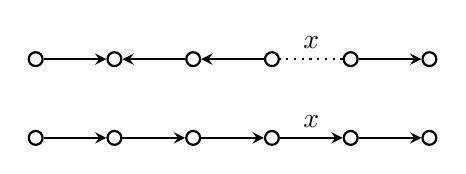
\begin{tikzpicture}
        \node[circle,draw,thick,minimum size=5pt,inner sep=0pt] (u1) at (0,0) {};
        \node[circle,draw,thick,minimum size=5pt,inner sep=0pt] (u2) at (1,0) {};
        \node[circle,draw,thick,minimum size=5pt,inner sep=0pt] (u3) at (2,0) {};
        \node[circle,draw,thick,minimum size=5pt,inner sep=0pt] (u4) at (3,0) {};
                                             
        \node[circle,draw,thick,minimum size=5pt,inner sep=0pt] (u5) at (4,0) {};
        \node[circle,draw,thick,minimum size=5pt,inner sep=0pt] (u6) at (5,0) {};

        \draw[thick,dotted,-] (u5) to node[midway,above] {$x$} (u4);
        \draw[thick,->] (u1) to (u2);
        \draw[thick,->] (u3) to (u2);
        \draw[thick,->] (u4) to (u3);
        \draw[thick,->] (u5) to (u6);

        \node[circle,draw,thick,minimum size=5pt,inner sep=0pt] (u1') at (0,-1) {};
        \node[circle,draw,thick,minimum size=5pt,inner sep=0pt] (u2') at (1,-1) {};
        \node[circle,draw,thick,minimum size=5pt,inner sep=0pt] (u3') at (2,-1) {};
        \node[circle,draw,thick,minimum size=5pt,inner sep=0pt] (u4') at (3,-1) {};
                                                                             
        \node[circle,draw,thick,minimum size=5pt,inner sep=0pt] (u5') at (4,-1) {};
        \node[circle,draw,thick,minimum size=5pt,inner sep=0pt] (u6') at (5,-1) {};

        \draw[thick,->] (u4') to node[midway,above] {$x$} (u5');
        \draw[thick,->] (u1') to (u2');
        \draw[thick,->] (u2') to (u3');
        \draw[thick,->] (u3') to (u4');
        \draw[thick,->] (u5') to (u6');
      \end{tikzpicture}

      
      \caption{Connecting two trees. The second figure shows the new graph after
        the insertion of $x$ to the position on its left.}
      \label{fig:cuckoo-insert-1}
    \end{marginfigure}

    In the figure, an arrow $u \to v$ indicates that the item corresponding to
    the edge $(u,v)$ is placed in position $u$ and its alternate location (given
    by $h_2$) is $v$. Since the two components are trees, we can direct the
    edges this way to create a DAG. Since every DAG has a sink node, there is
    some node in this graph which does not have an outgoing edge. Observe that a
    node is a sink iff there is no element in that position in the hash
    table. Thus, on inserting $x$, we could choose the position corresponding to
    $h_1(x)$, and the elements starting from the one in $h_1(x)$ will be moved
    until a sink in that directed graph is obtained. This requires $O(s)$-time
    in the worst case.
  \item If the two positions corresponding to $x$ lie in the same component,
    then the component is a tree, and adding $x$ into the hash table creates a
    single cycle in the cuckoo graph. This case is similar to the previous case
    since we can find the path to the sink in the directed version of the graph
    and move all the elements accordingly.
  \item The final case is when $x$ connects two components, one of which is a
    tree and the other contains exactly one cycle. If $h_1(x)$ belongs to the
    component containing the tree, then the insertion proceeds in the same way
    as the previous cases. The only thing to consider is when $h_1(x)$ belongs
    to the component containing the cycle. Firstly, observe that if we direct
    the edges like before, then we have directed cycle and edges directed
    towards the cycle (try to prove why this must be the case). See the figure
    on the right, for example.

    \begin{marginfigure}
      \centering
      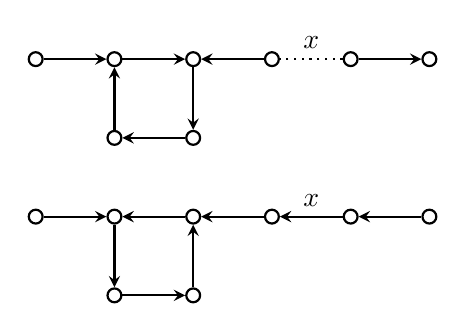
\begin{tikzpicture}
        \node[circle,draw,thick,minimum size=5pt,inner sep=0pt] (u1) at (0,0) {};
        \node[circle,draw,thick,minimum size=5pt,inner sep=0pt] (u2) at (1,0) {};
        \node[circle,draw,thick,minimum size=5pt,inner sep=0pt] (u3) at (2,0) {};
        \node[circle,draw,thick,minimum size=5pt,inner sep=0pt] (u4) at (2,-1) {};
        \node[circle,draw,thick,minimum size=5pt,inner sep=0pt] (u5) at (1,-1) {};
        \node[circle,draw,thick,minimum size=5pt,inner sep=0pt] (u6) at (3,0) {};
        \node[circle,draw,thick,minimum size=5pt,inner sep=0pt] (u7) at (4,0) {};
        \node[circle,draw,thick,minimum size=5pt,inner sep=0pt] (u8) at (5,0) {};
       
        \draw[thick,->] (u1) to (u2);
        \draw[thick,->] (u2) to (u3); \draw[thick,->] (u3) to (u4);
        \draw[thick,->] (u4) to (u5); \draw[thick,->] (u5) to (u2);
        \draw[thick,->] (u6) to (u3); \draw[thick,->] (u7) to (u8);
        \draw[thick,dotted,-] (u7) to node[midway,above] {$x$} (u6);

        \node[circle,draw,thick,minimum size=5pt,inner sep=0pt] (u1') at (0,-2) {};
        \node[circle,draw,thick,minimum size=5pt,inner sep=0pt] (u2') at (1,-2) {};
        \node[circle,draw,thick,minimum size=5pt,inner sep=0pt] (u3') at (2,-2) {};
        \node[circle,draw,thick,minimum size=5pt,inner sep=0pt] (u4') at (2,-3) {};
        \node[circle,draw,thick,minimum size=5pt,inner sep=0pt] (u5') at (1,-3) {};
        \node[circle,draw,thick,minimum size=5pt,inner sep=0pt] (u6') at (3,-2) {};
        \node[circle,draw,thick,minimum size=5pt,inner sep=0pt] (u7') at (4,-2) {};
        \node[circle,draw,thick,minimum size=5pt,inner sep=0pt] (u8') at (5,-2) {};
       
        \draw[thick,->] (u1') to (u2');
        \draw[thick,->] (u3') to (u2'); \draw[thick,->] (u4') to (u3');
        \draw[thick,->] (u5') to (u4'); \draw[thick,->] (u2') to (u5');
        \draw[thick,->] (u6') to (u3'); \draw[thick,->] (u8') to (u7');
        \draw[thick,->] (u7') to node[midway,above] {$x$} (u6');
      \end{tikzpicture}
      
      \caption{Inserting an element $x$ that connects a tree with a component
        with a single cycle. The second figure is the final connected component
        with the directions. Here $h_1(x)$ is the vertex to the left of $x$.}
      \label{fig:cuckoo-insert-2}
    \end{marginfigure}

    The insertion proceeds as follows: starting from $h_1(x)$, we will traverse
    the directed graph along the directed edges to the cycle, then traverse the
    cycle and come back to $h_1(x)$. When an edge $u\to v$ is traversed, the
    item in position $u$ is moved to the position $v$ and the direction of the
    edge changes. Once we reach back to $h_1(x)$, $x$ is moved to $h_2(x)$ which
    is in the other component (that is a cycle), and we keep moving until we
    reach a sink node like in the tree case. The each edge in the component
    containing the cycle is potentially traversed twice, and the total time is
    $O(s)$.
  \end{enumerate}
\end{proof}

We will now try to upper bound the size of connected components in the cuckoo
graph when $m$ items are inserted into a hash table of size $n$, where
$m = \tfrac{1-\epsilon}{2}n$. Since the hash functions are random, this is
equivalent to understanding the properties of the graph $G_{n,m}$, which is
uniform distribution over all graphs on $n$ vertices with $m$ edges. It turns
out that an easier graph to analyze is the Erd\"{o}-Renyi random graph $G_{n,p}$
which is the uniform distribution over graphs on $n$ vertices, where for each
pair of vertices, we add an edge with probability $p$, independently of all the
other pairs. \marginnote{You may note a similarity in the way we analyze
  $G_{n,p}$ instead of $G_{n,m}$ and approximating the balls-in-bins
  distribution using the Poisson distribution.}We will need to first show that
bounding the probability that there are no large components in $G_{n,p}$ (where
$p=m/\binom{n}{2}$) is sufficient to bound the probability that there are no
large components in $G_{n,m}$. We will assume for now that there are no
self-loops or edges in the graph sampled from $G_{n,m}$, since they cannot
increase the size of the connected components.

We will prove the following statements about the size of the connected
components in the cuckoo graph.
\begin{lemma}
  Let $G$ be a cuckoo graph with $n$ vertices and $m = \frac{1-\epsilon}{2} n$
  edges for some constant $\epsilon > 0$. Then, the following statements hold.
  \begin{enumerate}
  \item With probability $1 - 1/n$, the largest component in $G$ has size $O(\log n)$.
  \item The expected size of any connected component in $G$ is $O(1)$.
  \end{enumerate}
  \label{lem:cuckoo-cc}
\end{lemma}

Instead of proving this statement for graphs in $G_{n,m}$, we are going to prove
this for graphs in $G_{n,p}$. To that end, we will first show a connection
between the two graph distributions.

\begin{theorem}
  Let ${\cal P}$ be a any \emph{monotone graph property}. \marginnote{A monotone
    graph property is one where if $G\in {\cal P}$ and $G \subseteq G'$, then
    $G' \in {\cal P}$. For instance, connectivity is a monotone graph property.}
  Suppose that $P(n,m)$ and $P(n,p)$ be probability values defined as follows:
  \begin{align*}
    P(n,m) &= \Pr_{G\sim G_{n,m}}[G \in {\cal P}], \\
    P(n,p) &= \Pr_{G \sim G_{n,p}}[G \in {\cal P}]
  \end{align*}
  Let $p^{+} = (1+\epsilon)\frac{m}{\binom{n}{2}}$ and
  $p^- = (1-\epsilon)\frac{m}{\binom{n}{2}}$, for some constant $0 < \epsilon < 1$. Then,
  \begin{align*}
    P(n,p^-) - e^{-O(n)} < P(n,m) < P(n,p^+) + e^{-O(n)}
  \end{align*}
  \label{thm:random-graph-equiv}
\end{theorem}
\begin{proof}
  
\end{proof}

%%% Local Variables: 
%%% mode: latex
%%% TeX-master: "notes"
%%% End:

\chapter{Online algorithms}

This part of the course deals with \emph{online algorithms}. By this we mean that the input is revealed one at a time to the algorithm, and the algorithm must make an irrevocable decision every time it is revealed a part of the input. The algorithm does not have the benefit of hindsight to go back and correct a locally optimal decision it had made earlier. 

To measure the performance of such an algorithm, we calculate its \emph{competitive ratio}. This quantity measures the value output by the online algorithm on a particular sequence of input to the value that is output by the optimal algorithm for the same sequence. This optimal algorithm could even by offline, in the sense that it can make its decisions after seeing all the input. Formally, we define the notion of competitive ratio as follows.

\begin{definition}
	[Competitive ratio]
	An online algorithm $A$ for a computational problem $\mathcal{P}$ is
        said to have a competitive ratio of $c$ if for every input sequence
        $\sigma_1, \sigma_2, \ldots, \sigma_n$, the value return by $A$, given
        by $f_A(\sigma_1, \sigma_2, \ldots, \sigma_n)$ is such that
	\begin{align*}
          f_A(\sigma_1,\sigma_2,\ldots,\sigma_n) \leq c\cdot f_{\opt}(\sigma_1,\sigma_2,\ldots,\sigma_n).
	\end{align*}
	\label{def:comp-ratio}
\end{definition}

We will start with a small warm-up problem to set the stage.

\section{Warm up: Bipartite matching}

Let us start with the problem on online bipartite matching. In this problem, we have a bipartite graph $G(L\cup R, E)$ where the vertices in the set $L$ is known beforehand. The set of vertices in $R$ is revealed one at a time. When a vertex $v \in R$ is revealed, then all the neighbors $N(v)$ of $v$ are revealed. Let us start with a deterministic algorithm. We will see that the deterministic algorithm achieves a competitive ratio of $1/2$, and that this is the best ratio achievable by any deterministic algorithm.

Consider the following greedy algorithm. When a new vertex $v$ is revealed with the edges, choose an edge arbitrarily that can be included in the current matching. We start with the the empty matching. Note that this algorithm is the greedy algorithm to construct a maximal matching.

\begin{theorem}
	The greedy algorithm for maximal matching is $2$-competitive.
	\label{thm:maximal}
\end{theorem}
\begin{proof}
	If $M$ is a maximal matching and $M^\star$ is a maximum matching, we will see that $|M^\star| \leq 2|M|$. This follows from the following two observations.
	\begin{enumerate}
		\item For every edge $(u,v) \in M^\star - M$, one of the edges incident on $v$ or $u$ must be in the maximal matching, since otherwise $M$ cannot be maximal.
		\item For every edge $(u,v) \in M - M^\star$, at most $2$ edges incident on $u$ and $v$ can be in the maximum matching $M^\star$.
	\end{enumerate}
	Both the observations together imply that $|M^\star| \leq 2|M|$.
\end{proof}

We can also see that this is the best ratio achievable by any deterministic online algorithm for bipartite matching. To see this, consider the graph where $L$ consists of two vertices $u_1, u_2$. Now the first vertex $v_1$ in $R$ that comes is connected to both $u_1$ and $u_2$. No matter which edge the deterministic algorithm chooses in the matching, say $(u_1, v_1)$, the next vertex $v_2$ will be connected to $u_1$. So, the graph looks as follows.

Clearly, the maximum matching is of size $2$, whereas the deterministic algorithm gives a matching of size $1$.

Online bipartite matching is a special case of a more general problem that has received a lot attention in recent years. This is the AdWords problem. Consider the way a company like Google generates the revenue through ads. Whenever a user searches a keyword, the search engine displays a bunch of ads related to the searched keywords together with the search results. If the user clicks on any of the ads, the entity that displays the ad pays Google some revenue. This is modelled as follows: There is a set of $n$ sellers that are known beforehand. Whenever a new keyword is searched, the $n$ sellers provide the bid for that item. The job of the search engine is to assign that keyword to one of the sellers whose ad will be displayed. Each keyword can be assigned to at most one seller, and the aim of the search engine is to maximize its revenue. The sellers are constrained by a budget, and hence cannot be assigned keywords such that the sum exceeds its budget. Bipartite matching is a special case, where each seller has unit budget, and make a $0-1$ bid for every keyword that appears.

We will see that if we allow randomization, then online bipartite matching has an algorithm with competitive ratio $1 - 1/e$. Furthermore, this is the best that can be achieved by any online algorithm for bipartite matching. We will see this a little later.

\section{Online paging}

Consider the problem of maintaining a cache memory of size $k$ in response to a sequence of requests. If the request corresponds to a page already present in the cache, then it can be serviced quickly and is known as a \emph{hit}. If the request is not present in the cache, then the page has to be brought in from say the main memory, which is a slow memory, into the cache. This is known as a \emph{cache miss} or a \emph{fault}. At every cache fault, we must necessarily evict an item from the cache to make room for the new item. The goal is to design a scheme that chooses the best item to evict so that the number of cache faults is minimized. It is not hard to see that for any deterministic online paging algorithm, it is possible to construct a sequence of request adversarially such that the algorithm faults on every request. We will see this when we prove lower bounds on the competitive ratio of paging algorithms.

\subsection{Deterministic online paging}
First, we will start with some deterministic algorithms. A simple algorithm, that is also used a lot in practice, is the LRU (Least-Recently-Used) scheme. In this algorithm, whenever a request for a page that is not in the cache comes, we choose the page that was requested farthest in the past to evict. We will see that LRU is $k$-competitive, and that any deterministic algorithm that is $c$-competitive must have $c \geq k$. What does an optimal (possibly offline) algorithm for paging look like? This is obtained by the LFD (Longest-Future-Distance) scheme, where we choose the item that will be requested farthest in the future to be evicted in case of a cache fault. Notice that this is necessarily an offline algorithm.

\begin{theorem}
	The LRU algorithm is $k$-competitive.
	\label{thm:paging-det-ub}
\end{theorem}
\begin{proof}
	We will divide the sequence of requests $\sigma_1,\sigma_2,\ldots,\sigma_n$ into rounds where a round is a maximal set of requests that generate $k$ cache misses for the LRU algorithm. We will then show that in each round, the optimal algorithm must fault at least once. This will prove the bound on the competitiveness ratio.
	
	Consider an arbitrary round $i$. We will consider two cases.
	\begin{enumerate}
		\item Case 1: There is a page $\sigma_j$ that generated two faults in round $i$. Consider the sequence between these two faults for $\sigma_j$. The reason for the second fault is that even though $\sigma_j$ was brought into the cache, it was evicted at some later stage. Since LRU evicts a page that was requested farthest in the past, this means that there must have been at least $k-1$ different requests before $\sigma_j$ was evicted. Hence, in round $i$ there must have been at least $k+1$ different requests - one for the first $\sigma_j$ request, then the $k-1$ other requests before $\sigma_j$ was evicted, and finally the request for $\sigma_j$ that brought it back into the cache. Since the cache size is only $k$, no matter what the optimal algorithm does it must fault at least once on $k+1$ requests.
		\item Case 2: Suppose that all the $k$ faults in round $i$ were for distinct items. Now let $\sigma_i$ be the last request in round $i-1$. Notice that the page $\sigma_i$ is present in the cache for the LRU algorithm and the optimal algorithm. Suppose that $\sigma_i$ was not one of the $k$ faults in round $i$. This means that there are $k$ distinct page requests other than $\sigma_i$, and hence the optimal algorithm must fault at least once. 
		
		On the other hand, if $\sigma_i$ was one of the $k$ distinct faults. This means that on one of the requests in round $i$, $\sigma_i$ was evicted. Since LRU evicts the least recently used element, and $\sigma_i$ was the last request in round $i-1$, there must have been at least $k-1$ different requests before that. Together with the request that evicted $\sigma_i$ and the request for $\sigma_i$ that generated a miss, this means there were $k+1$ distinct requests in round $i$. Hence, the optimal algorithm must have faulted at least once.
	\end{enumerate}
\end{proof}

We will now see that this is the best achievable if we restrict ourselves to deterministic algorithm. The idea is to show that given a deterministic algorithm, we can always generate a sequence of requests that forces the algorithm to miss on every request. 

For concreteness let $A$ be a fixed deterministic online paging algorithm, and suppose we start with a cache with $k$ items. The first request will be an element that is not one of these elements. Thus, we have a set $S$ of $k+1$ elements such that every request will be an item from this set. In particular, the $i^{th}$ request will be the elements currently not in the cache according to the algorithm $A$. Thus, the algorithm has a cache miss on each of the requests. To understand the behaviour of the optimal algorithm, let us divide the request sequence into rounds where a round is a maximal sequence of requests that contain $k$ distinct requests. Note that $A$ has at least $k$ faults in a round. Let us now argue that the optimal algorithm (LFD) will miss at most once in a round. 

Since a round contains $k$ distinct requests, there is some element in $S$ that was never requested in that round. The optimal algorithm will then evict that item at the first miss in the round. This guarantees that there are no more misses in that round. Thus, we have shown the following.

\begin{theorem}
	Any $c$-competitive deterministic paging algorithm must have $c \geq k$.
	\label{thm:paging-det-lb}
\end{theorem}

\subsection{Randomized online paging}

In this part, we will see that randomized algorithms can achieve better guarantees on the competitive ratio. To study randomized algorithms, we need a suitable way to define the competitive ratio. Notice that in the case of a deterministic algorithm, the adversary who constructs the requests have complete information about the algorithm, and hence can tell clearly the request that the algorithm will make in any step.

In the case of a randomized algorithm, the algorithm has access to random coins. Now, even if the adversary knows the randomized algorithms, it might still not know the exact sequence of the pages evicted by the algorithm since that also depends on the random coins of the algorithm. This can potentially mean that we have an algorithm that has a better competitive ratio. To formalize this notion, let us define what an \emph{oblivious adversary} is.

We can think of an oblivious adversary as someone who knows the randomized algorithm, but has no access to the random coins that is used by the algorithm in its execution. Thus we can think of an oblivious adversary looking at the source code of the randomized algorithm and generating a sequence of requests. The oblivious adversary then runs the optimal (possibly offline) algorithm on this sequence. Notice that the outcome of the optimal algorithm is deterministic. But now, the outcome of the online algorithm is a random variable that depends on its internal coin tosses. Like before, we say that a randomized online algorithm has a competitive ratio of $c$ if there is a $\delta$ such that for every sequence $\sigma_1, \sigma_2, \ldots, \sigma_n$, we have
\begin{align*}
	\E(f_A(\sigma_1,\sigma_2,\ldots,\sigma_n)) \leq c. f_{\opt}(\sigma_1, \sigma_2, \ldots, \sigma_n).
\end{align*}
Here the expectation is over the internal coin tosses on the algorithm $A$. We will show that there is an online paging algorithm with a competitive ratio of $2H_k$, and that there is an almost matching lower bound. First we will describe the randomized paging algorithm.

This is known as the \marker algorithm. In this algorithm, we have a marker bit associated with each cache location. The algorithm is divided into rounds. Each round start with the marker bits all set to $0$. When a cache request comes, if the element is present in the cache, the corresponding bit is set to $1$, if it is not already so. If the request is a miss, we choose a location uniformly at random from all the positions whose bits are $0$, evict that item and put the new item in that location. The corresponding bit is set to $1$. Once all the bits are set to $1$, the round is completed when a cache request to an item not currently in the cache arrives. At this stage all the marker bits are set to $0$, and the next round starts.

\begin{theorem}
	The \marker algorithm is $2H_k$-competitive.
	\label{thm:rand-paging-ub}
\end{theorem}
\begin{proof}
	Our analysis is quite similar to what we saw earlier. We will divide the sequence of requests into rounds, then give an upper bound on the expected number of cache misses by the \marker algorithm and lower bound for the number of misses by the optimal algorithm. Here the notion of a round is what is defined by the \marker algorithm. In a particular round $i$, let $I_O$ denote the items that were requested in round $i$ and in round $i-1$, and let $I_N$ denote the items that were requested in round $i$, but not in round $i-1$. 
	
	Firstly, note that for each item in $I_N$, the \marker algorithm will fault. This is because round $i-1$ ended when the first request to an element not in cache arrived with all the marker bits set to $1$. The only way a marker bit is set to $1$ is when that particular element is requested. Once the marker bit is set to $1$, the corresponding element is never evicted in that round. 
	
	Our aim is to find the expected number of elements in $I_O$ that faults in round $i$. Consider the $j^{th}$ element in $I_O$ when it is first requested in round $i$. Now, the positions where the first $j-1$ elements of $I_O$ were occupied at the start of round $i$ have their bit set to $1$ since either one of the $j-1$ elements is already present there and was requested, or it was evicted and a new element from $I_N$ is placed there and the bit is set to $1$. So, out of the at most $|I_N| + j - 1$ distinct requests preceding the request for the $j^{th}$ item in $I_O$, $j-1$ requests have been placed in the position corresponding to the first $j-1$ elements in $I_O$. The remaining at most $|I_N|$ requests are placed in the remaining $k - j + 1$ positions, one of which is the position where item $j$ is. Therefore, the probability that there is a cache miss on item $j$ is at most $|I_N|/(k - j + 1)$. Let us call $|I_N| = n_i$, the number of new requests in round $i$. Thus, we have the probability of a cache miss on item $j$ to be $n_i/(k-j+1)$.
	
	Thus the expected number of cache misses in round $i$ of the algorithm is given by
	\begin{align*}
		n_i + \sum_{j=1}^{k-n_i} \frac{n_i}{k-j+1} &= n_i + n_i\sum_{\ell = n_i + 1}^k \frac{1}{\ell}\\
		&= n_i + n_i(H_k - H_{n_i})\\
		&\leq n_i H_k.
	\end{align*}
	The total number of misses across the entire request sequence is therefore $H_k \sum_{i=1}^p n_i$ where $p$ is the number of rounds.
	
	Now, let us look at the case of the optimal paging algorithm and the number of its cache misses. Consider a round $i$, and let $n_i$ be the new items that were requested in round $i$. Suppose that $d_i$ was the number of elements present in the cache of the offline algorithm that are not present in the cache of the \marker algorithm at the start of a round $i$. This means that the offline algorithm has at least $n_i - d_i$ cache misses in round $i$. Similarly, the offline algorithm has $d_{i+1}$ elements in the cache after round $i$ that are not in the \marker algorithm. Now, every element in the cache of the \marker algorithm was requested in round $i$. So, if there are $d_{i+1}$ elements in the offline algorithm that are not in the cache of the \marker algorithm, there must have been at least $d_{i+1}$ cache misses for the offline algorithm. So, we can say that the number of cache misses in round $i$ is at least $(n_i - d_i + d_{i+1})/2$. At the start of round $1$, both the algorithms start with the same cache content, and hence $d_1 = 0$. Thus the total number of cache misses by the offline algorithm is at least $(\sum_{i=1}^p n_i)/2$, and this gives the $2H_k$ bound on the competitive ratio.
\end{proof}

\section{Yao's minimax principle and lower bounds}

We will now see a generic method to prove lower bounds against randomized models of computation, and use it to show that any paging algorithm must have a competitive ratio of at least $H_k$. 

Consider a \emph{two-player zero-sum game} between a row player $(R)$ and a column player $(C)$. By a zero-sum game, we mean that every play has a winner and an associated payoff that the loser gives to the winner. Such a game can be characterized by an $m\times n$ matrix $M$ known as the \emph{payoff matrix}. The $m$ rows of $M$ correspond to the actions of $R$, and the $n$ columns of $M$ correspond to the actions of $C$. Then entry $M_{ij}$ corresponds to the payoff that $R$ received from $C$ when $R$ plays $i$ and $C$ plays $j$. For instance, the classical rock-paper-scissors game can be characterized by the following payoff matrix: $-1$ indicates that the column player wins and the row player has to pay the payoff to the column player.
\begin{align*}
\begin{blockarray}{cccc}
	& Rock & Paper & Scissors \\
	\begin{block}{c[ccc]}
		Rock & 0 & -1 & 1 \\
		Paper & 1 & 0 & -1 \\
		Scissors & -1 & 1 & 0 \\
	\end{block}
\end{blockarray}
\end{align*}

What would a good strategy for $R$ look like? There are $3$ possible actions, and for each there is a minimum payoff that he/she receives irrespective of the actions of the player $C$. If $R$ is unaware of the actions of $C$, then the best possible strategy for $R$ is to choose the action that maximizes the minimum payoff that he/she can receive. Similarly for the column player $C$, he/she plays the action that minimizes the maximum payoff that $C$ has to pay $R$ among all his/her actions. The game is said to have a value if 
\begin{align*}
	\max_{i} \min_{j} M_{ij} = \min_{j} \max_{i} M_{ij}.
\end{align*}
In other words, if there exists such an action, then this is the best possible strategy for either of the players if they do not now know the action of the other player. Notice that not all games have such a value - see the example of the rock-paper-scissors game. There $\max_{i} \min_{j} M_{ij} = -1$ and $\min_{j} \max_{i} M_{ij} = 1$.

In particular, it is possible to observe the following statement.
\begin{lemma}
	For every payoff matrix $M$ of a two-player zero-sum game, we have
	\begin{align*}
		\max_{i} \min_{j} M_{ij} \leq \min_{j} \max_{i} M_{ij}.
	\end{align*}
	\label{lem:pure-strat}
\end{lemma}

A strategy where the player choose a fixed action is known as a \emph{pure strategy}. What we have seen is that there need not exist an equilibrium pure strategy for the game. On the other, if we look at \emph{mixed strategies}, then indeed such equilibriums exist. A mixed strategy is a probability distribution over the actions of the corresponding player. The player then chooses an action according to this probability distribution. 

Consider a distribution $\dist{p}$ over the rows of $M$, and a distribution $\dist{q}$ over the columns of $M$. Now, instead of looking at the payoff directly, we will be interested in the expected payoff. This can be easily seen to be
\begin{align*}
	\sum_{i=1}^m \sum_{j=1}^n p_i q_j M_{ij} = \dist{p}^TM\dist{q}.
\end{align*}
Like in the case of pure strategies, the goal of the row player is to choose a distribution $\dist{p}$ such that irrespective of the mixed strategy of $C$, the expected payoff is maximized. But, unlike in the case of pure strategies, there is always an equilibrium for mixed strategies. 
\begin{theorem}[von Neumann Minimax Theorem]
	Let $M$ be a payoff matrix for a two-player zero-sum game. Then,
	\begin{align*}
		\max_{\dist{p}} \min_{\dist{q}} \dist{p}^T M \dist{q} = \min_{\dist{q}} \max_{\dist{p}} \dist{p}^TM\dist{q}.
	\end{align*}
	\label{thm:vn-minimax}
\end{theorem}

Notice that if $\dist{p}$ is fixed, then $\dist{p}^TM \dist{q}$ is a convex sum of the elements of the row vector $\dist{p}^TM$. Consequently, the distribution $\dist{q}$ that minimizes the inner product is the one that puts all the mass on the index with the smallest value. Thus, we have a simply corollary to the minimax theorem that we will use to build the framework for our lower bound proofs.

\begin{corollary}
	Let $M$ be a payoff matrix for a two-player zero-sum game. Then,
	\begin{align*}
		\max_{\dist{p}}\min_j \dist{p}^TM\dist{e}_j = \min_{\dist{q}}\max_i \dist{e}_i^TM \dist{q}.
	\end{align*}
\end{corollary}

Yao's minimax principle is essentially a restatement of the minimax theorem, when a randomized algorithm is viewed as a game. We can think of a game between an algorithm designer and an adversary in the following way: the aim of the designer is to come up with an algorithm that has good performance guarantees on every input, whereas the goal of the adversary is to come up with an input where the algorithm fares poorly. We can think of this as a zero-sum game with a payoff matrix where rows are indexed by the inputs $\mathcal{I}$ and the columns are indexed by algorithms $\mathcal{A}$. The value $M_{ij}$ is the cost of the algorithm $A_j$ on the input $I_i$. For caching algorithms, the cost will be the number of cache misses for the caching algorithm $A_j$ on the input sequence $I_i$.

Observe that we can think of a randomized algorithm as a distribution $\dist{a}$ over the set of all deterministic algorithms on inputs of length $n$, say. Thus, the minimax theorem tells us that 
\begin{align*}
	\max_{\dist{i}} \min_{\dist{A}} \E_{\substack{A\sim \dist{a}\\ I\sim \dist{i}}}[c(A,I)] = \min_{\dist{a}} \max_{\dist{i}} \E_{\substack{A\sim \dist{a}\\ I\sim \dist{i}}}[c(A,I)].
\end{align*}
where $c(A,I)$ is the number of misses for the deterministic algorithm $A$ on the input $I$. Furthermore, from the corollary of the minimax theorem, we can say that
\begin{align*}
	\max_{\dist{i}} \min_A \E_{I\sim \dist{i}} [c(A,I)] = \min_{\dist{a}} \max_I \E_{A\sim \dist{a}} [c(A,I)].
\end{align*}
From this, we can conclude the following about any distribution $\dist{a}$ and $\dist{i}$.
\begin{align*}
	\min_A \E_{I\sim \dist{i}}[c(A,I)] \leq \max_I\E_{A\sim \dist{a}}[c(A,I)].
\end{align*}
Notice that the right-hand side of the inequality is the worst-case expected number of cache misses for a randomized algorithm $\dist{a}$, and the left-hand side is the minimum number of expected misses for any deterministic paging algorithm when the input sequence is distributed according to $i$. Thus, we can conclude the following, which is referred to as Yao's minimax principle.
\begin{theorem}[Yao's minimax principle]
	Suppose there exists a distribution $\dist{i}$ over inputs such that every deterministic algorithm incurs an expected cost (over the input distribution) of $c$. Then, any randomized algorithm will incur an expected cost of at least $c$.
	\label{thm:yao}
\end{theorem}

We will now apply Yao's minimax principle to obtain a lower bound on the expected number of cache misses for any paging algorithm.

\subsection{Lower bound for online paging}

We will prove the following theorem in this subsection. The idea is to design a distribution over inputs such that every deterministic paging algorithm will incur a large number of cache misses in expectation, and conclude using the minimax principle. 

\begin{theorem}
	If an online algorithm for paging (randomized or deterministic) is $c$-competitive, then $c \geq H_k$.
	\label{thm:lb-pagin}
\end{theorem}
\begin{proof}
	We start by defining a distribution over inputs such that any deterministic paging algorithm will incur a large cost. Let $S$ be the set of elements in the cache at the start, and let $i$ be some element that is not present in the cache. Our cache request will be from the set $I = S \cup \{i\}$. The first request will be the element $i$. Thereafter, if the current request was $\sigma_i$, then the next request will be an item chosen uniformly at random from $I \setminus \sigma_i$. 
	
	Once again, we will divide the request sequence into rounds where a round consists of $k$ distinct requests, and end just before the $k+1^{st}$ distinct element is requested. We will argue that any deterministic algorithm will have at least $H_k$ cache misses, whereas the optimal algorithm will have at most one cache miss per round. 
	
	The bound for the optimal algorithm is essentially the same as what we saw before. Since the $k+1^{st}$ distinct element is requested only in the next round and since all the requests are from a set of $k+1$ elements, we can evict the $k+1^{st}$ if there is a cache miss. Now we can be sure that there will be no more cache misses in the current round.
	
	For any deterministic algorithm, the state of the algorithm at a step $i$ of the request sequence is fully characterized by the element not present in the cache at that point. The deterministic algorithm will have a cache miss iff the next element in the sequence is the element that is outside the cache. Since we never request the same element twice in a row, and the requested element is chosen at random from the remaining elements, the probability of a cache miss is $1/k$. To complete, we need to bound the expected length of a round.
	
	To do this, think of the complete graph on the vertex set $I$. At the beginning of a round we are at a vertex $v \in I$, and every request consists of choosing random neighbor and moving to that neighbor. The round ends precisely when we have visited every vertex in the graph. Once we have visited $i$ vertices, the probability that the next vertex will be an unvisited vertex is $(k-i+1)/k$. Thus the expected number of steps before visiting and unvisited vertex is $k/(k-i+1)$. Thus, similar to the bound on the coupon collector problem, we can conclude that the expected length of a round is $kH_k$. This concludes the argument that the expected number of cache misses for any deterministic algorithm is at most $H_k$ per round.
\end{proof}

\section{Bipartite matching revisited}

Let us go back to the online bipartite matching problem. We will start with an observation that any deterministic algorithm for online bipartite matching cannot achieve a competitive ratio better than $2$. This follows from the following simple example. Suppose that $L$ consists of two vertices $u_1$ and $u_2$. Now, the first vertex in $R$ is $v_1$ and its edges are $(u_1, v_1)$ and $(u_2, v_1)$. The online algorithm must choose one of these edges in the matching, say $(u_1, v_1)$. Now, the adversary will reveal $v_2$ with the edge $(u_1, v_2)$. This edge cannot be added to the matching and hence the size of the matching obtained is $1$ whereas the best offline algorithm gives a matching of size $2$. 

The bipartite matching problem is a special case of a more general problem known as the AdWords problem, where you have a set of sellers $L$ and a set of keywords $K$. Each seller $l_i$ has a valuation $v_j$ for the $j^{th}$ keyword - this is the amount the seller is willing to pay for their ad to be displayed when the keyword is searched. Now, the keywords come online and the valuations for each of the sellers for that keyword is revealed. You have to assign the keyword to a seller and you receive the revenue you receive is the valuation of that keyword given by the seller. Your goal is to maximize the revenue, subject to the constraint that every seller has a budget beyond which he/she is not willing to buy a keyword. It is easy to see that the bipartite matching problem is an instance of the AdWords problem when each seller has unit budget and has a valuation that is either $0$ or $1$ for every keyword.

We will now see a randomized online algorithm for bipartite matching that achieves a competitive ratio of $1 - 1/e$. It can also be shown using the minimax principle that this is the best bound achievable by any online algorithm. We now describe this algorithm, \ranking, first described by Karp, Vazirani and Vazirani.

\begin{algorithm}[h]
	\KwIn{$G(L,R,E)$, where $L$ is known and $R$ is revealed online}
	
	Choose a permutation $\pi$ uniformly at random and order vertices of $L$ according to $\pi$
	
	$M \gets \emptyset$
	
	\ForEach{$v\in R$ and its neighbors $N(v)$ revealed online}{
		Find the first vertex $u \in N(v)$ (according to $\pi$) that is unmatched
		
		$M \gets M \cup \{u,v\}$
	}
	\label{alg:ranking}
	\caption{\ranking}
\end{algorithm}  

We will show that the matching computed by \ranking is a $1-1/e$-approximation of a maximum matching. More precisely, we will show that the expected size of the matching computed by \ranking (where the expectation is over the random permuation in Step~$1$) is at least $(1-1/e)\cdot \opt$, where $\opt$ is the size of the maximum matching.

To that end, we will view this algorithm as a market process between buyers and items. Let $L$ be a set of items such that each item $i$ has a price $p_i$. Now, $R$ consists of a set of buyers where each buyer $j$ has a valuation $v_j(i)$ for each item item $i \in N(j)$. The utility of an item $i$ for a buyer $j$, denoted by $u_j(i) = v_j(i) - p(i)$. The buyers arrive in an online fashion, and buyer $i$ purchases the item with the highest utility in $N(i)$ that has not yet been sold. We will assume that the prices are set in a randomly, by first sampling a number $w$ uniformly at random from the interval $[0,1]$ and setting the price $p_i$ to be $e^{w-1}$. The valuation $v_j(i)$ is set to $1$ for each buyer $j$ and item $i$. 

Since we are sampling from a distribution with no point mass, there are no two prices that are same, and it induces an ordering on the items in $L$. Thus, the market process corresponds to running the \ranking algorithm with the permutation corresponding to what is given by the prices. In other words, if $M$ is the matching given by the \ranking algorithm and $M'$ the matching given by the market process, we have
\begin{align*}
	\E_\pi [M] = \E_w[M'].
\end{align*}

To analyze this algorithm, let us first write the size of the matching given by the market process using the utility obtained by the buyers and the revenue generated. For a price list $\dist{w}$ generated as above, let us define the utility for the user $i$ to be $1 - p_j$ if the user has bought item $j$ and $0$ otherwise. For an item $j$, we will define the revenue to be $r_j$ is the item was purchased during the market process. Observe that we can write the size of the matching $M'$ as follows:
\begin{align*}
	|M'| = \sum_{i\in L} r_i + \sum_{j\in R} u_j
\end{align*}
Let $M^*$ be a maximum matching, we can then write
\begin{align*}
	\E[|M'|] &= \E\left[\sum_{i\in L} r_i + \sum_{j\in R} u_j \right] \geq \E\left[ \sum_{(i,j)\in M^*} (r_i + u_j) \right]\\
	&= \sum_{(i,j)\in M^*} \E[r_i + u_j]
\end{align*}

To complete the proof, we need to prove the following claim.
\begin{claim}
	Let $(i,j)$ be any edge in the graph $G$. Then $\E[r_i + u_j] \geq 1 - 1/e$.
\end{claim}
\begin{proof}
	Consider the same market process with the same sequence except the item $i$. Let $M'_i$ be the matching generated by the market process in this case. Let $p^* = e^{w^* - 1}$ be the price of the item purchased by the buyer $j$ in $M'_j$. If $j$ does not purchase any item, then set $p^* = 1$. 
	
	Notice that if $p_i < p^*$, then the item $i$ is purchased by some buyer in $M'$. This is because if it was not purchased by the time buyer $j$ arrives, then the utility $u_j(i) = 1 - p_i > 1 - p^*$ and hence $j$ will purchase $i$. Furthermore, the utility of $j$ in $M'$, $u_j > 1 - p^*$ since adding a new item cannot reduce the utility. Therefore, $\E[u_j] > 1 - p^*$. 
	
	Now $\E[r_i] = \E[p_i I_[\text{$i$ is purchased}]] \geq \E[p_i I[p_i < p^*]]$. The final inequality follows from the first observation in the last paragraph. Thus, we can write
	\begin{align*}
		\E[r_i] \geq \int_{0}^{w^*} e^{w-1} dw = p^* - \frac{1}{e}.
	\end{align*}
    Thus, we have $\E[r_i + u_j] \geq 1 - 1/e$ and this concludes the proof.
\end{proof}

\section{The Multiplicative Weights Update (MWU) method}

In this part we will look at a generic meta-algorithm known as the multiplicative weights update (MWU) method. The method is fairly elementary, but very many different algorithms can be seen as instantiations of this meta-algorithm. We start with an  online decision making problem.

\subsection{The weighted majority algorithm}

Consider a decision making problem where you have to make a yes/no decision everyday, and if you make the wrong decision you have to pay a thousand rupees to an adversary. If you make the correct decision, then you do not have to pay anything. Now, the catch is that the adversary can reveal to you the correct answer only after you say your decision. Clearly, this game is loaded in favor of your adversary for he/she can force you to pay up at every step.

Now consider the case that there are $n$ experts $e_1, e_2, \ldots, e_n$ whom you can listen to while making a decision. Instead of measuring your performance in the worst-case scenario, you would like to measure it in terms of the performance of the best experts among the $n$. In other words, we are interested in the quantity
\begin{align*}
	\min_{i\in [n]} \{ m^{(i)}_T \} - m_T,
\end{align*}
where $m^{(i)}_T$ is the number of times that the $i^{th}$ expert made a wrong decision and $m_T$ is the number of times you made the wrong decision in $T$ steps. We would like to make this as small as possible. Let us start with a simple warm-up that we will generalize.

\subsection{Omniscient expert}

Assume that among the $i$ experts, there exists an omniscient expert who can make the correct decision every time. We will see we can find the identity of such an expert in $\log n$ steps where we made an incorrect decision, and hence $\min_{i\in [n]} \{ m^{(i)}_T \} - m_T \leq \log n$. The idea is that at every step we take the majority decision of the remaining experts, and once the correct decision is revealed we throw away all the experts who gave incorrect answers at that stage. The omniscient expert is never thrown away, and furthermore if we make an incorrect decision, this means that at least half of the experts in that stage can be identified as bad experts and thrown away.

\subsection{General case}

In the general case, there need not be any omniscient expert. We also cannot make any assumptions on how the experts are correlated. For instance, maybe there is a clique of $k$ experts who always give the same answer. The idea of the weighted majority algorithm is fairly simple. Initially, we are unaware of which of the experts really know what they are talking about. So, we trust each of their decisions equally well. But then once we see how they fare, we factor that in and re-weight our trust in the experts. This is described in Algorithm~\ref{alg:wgtd-maj}.

\begin{algorithm}%[h]
	Set $w_i^{(1)} \gets 1$ for every $i \in [n]$
	
	\For{$t = 1$ to $T$}{
		Let $S_0$ be the experts who say no, and let $S_1$ be the expert who says yes.
		
		\leIf{$\sum_{i\in S_0} w_i^{(t)} \geq \sum_{i\in S_1} w_i^{(t)}$}{
			decide no
		}{
			decide yes
		}
		
        \ForEach{wrong expert $i$}{set $w_i^{(t+1)} \gets (1-\epsilon)w_i^{(t)}$}
	}
	\caption{\textsc{Weighted Majority}}
	\label{alg:wgtd-maj}
\end{algorithm}

In the first step we take the majority vote, but after that we scale down the weight of wrong experts. The factor $\epsilon$ in the algorithm is a weighting factor that decides by how much we should rescale a wrong experts advice. We can show that this simple algorithm already achieves almost the best that we can achieve by deterministic algorithms.

\begin{theorem}
	Let $m_T$ be the number of mistakes made by the weighted majority algorithm after in $T$ steps, and let $m^{(i)}_T$ be the number of mistakes made by expert $i$ in $T$ steps. Then, for every $i \in [n]$ we have
	\begin{align*}
		m_T \leq 2(1+\epsilon)m^{(i)}_T + \frac{\log n}{\epsilon}.
	\end{align*}
	\label{thm:wgtd-maj}
\end{theorem}
\begin{proof}
	The proof is similar in spirit to the case of the omniscient expert. Let us define a potential function $\Phi(t) = \sum_{i=1}^n w_i^{(t)}$. We will show that at each time step that we make an erroneous decision the potential function reduces by a constant factor.
	
	Firstly, notice that for any expert $i$, we have $w_i^{(t)} = (1-\epsilon)^{m_T^{(i)}}$. If at time step $t$, the algorithm makes a wrong decision (say the algorithm said no w.lo.g), then we can write
	\begin{align*}
		\Phi(t+1) &= \sum_{i\in S_0} w_i^{(t+1)} + \sum_{i\in S_1} w_i^{(t+1)}\\
		&= (1-\epsilon)\sum_{i\in S_0} w_i^{(t)} + \sum_{i\in S_1} w_i^{(t)}\\
		&\leq \left( 1 - \frac{\epsilon}{2}\right)\Phi(t).
	\end{align*}

	Thus, after $T$ steps, for every $i\in [n]$ we have
	\begin{align*}
		(1-\epsilon)^{m_i{(T)}} \leq \Phi(T) \leq \left(1 - \frac{\epsilon}{2} \right)^{m_T}n
	\end{align*}
	The bound follows from taking logarithm on both sides and using the approximation for $\ln(1-x)$.
\end{proof}

%%% Local Variables: 
%%% mode: latex
%%% TeX-master: "notes"
%%% End:



\end{document}

